\documentclass[conference]{IEEEtran}
\usepackage{cite}
\usepackage{amsmath,amssymb,amsfonts}
\usepackage{algorithmic}
\usepackage{graphicx}
\usepackage{textcomp}
\usepackage{xcolor}
\usepackage{hyperref}
\usepackage{float}
\usepackage{tikz}
\usetikzlibrary{matrix,calc}
\usepackage{graphicx}
\usepackage{color,soul}
\usepackage{svg}
\usepackage{subfigure}
\usepackage{mdframed}
\usepackage{natbib}
\usepackage{verbatimbox}
\usepackage{tkz-euclide}
\usepackage{listings}
\usepackage{mathtools}
\usepackage{xcolor}
\usepackage[hyphens]{url}
% \usepackage[hidelinks]{hyperref}
% \hypersetup{breaklinks=true}
% \urlstyle{same}
\usepackage{cite}


\usepackage{etoolbox}
\AtBeginEnvironment{quote}{\par\singlespacing\small}

\usepackage[toc,page]{appendix}

\lstset{language=C++,
        basicstyle=\ttfamily\small,
        keywordstyle=\color{blue}\ttfamily\small,
        stringstyle=\color{red}\ttfamily\small,
        commentstyle=\color{green}\ttfamily\small,
        morecomment=[l][\color{magenta}]{\#}
}


\def\BibTeX{{\rm B\kern-.05em{\sc i\kern-.025em b}\kern-.08em
    T\kern-.1667em\lower.7ex\hbox{E}\kern-.125emX}}
\begin{document}

\title{Augmenting the guitar as an MPE controller with capacitive touch sensors}

\author{\IEEEauthorblockN{Jamie R. Pond}
\IEEEauthorblockA{\textit{School of Electronic Engineering and Computer Science} \\
\textit{Queen Mary, University of London}\\
London, United Kingdom \\
ec20768@qmul.ac.uk}
}

\maketitle

\begin{abstract}

We explore the development of a prototype MIDI Polyphonic Expression (MPE) enabled, guitar-like instrument for use in the modern music production studio. Following a process of human-centred design and human-computer interaction, we focus on creating a prototype that is conducive to fostering creative flow. This is achieved through the implementation of capacitive touch sensors (Bela Trill Bar) which are affixed to the frets of the prototype, which offers affordances of polyphonic aftertouch and pitch bend. The data thereof is interpreted with a given mathematical and programming framework. We find that the prototype is proficient at supporting novel creative musical ideas and subjectively pleasingly idiosyncratic musical performances, however this is somewhat impeded by practical prototyping choices. 

A brief demonstration of the working prototype is  \href{https://drive.google.com/file/d/1nzG5n9ZV4Jj0LsfHVGwRh3t7zOLOUAXv/view?usp=sharing}{\textit{available here}}.


% In this paper we will explore the development of a prototype MIDI Polyphonic Expression (MPE) enabled digital instrument. This work focuses on the process of human-centred design and human-computer interaction with a focus on creating instruments that are not only conducive to fostering flow in musicians, but also ensuring an accessible design for blind, limb-different and left-handed users. This work also attempts to tackle the stigma of digital instruments that has been highlighted in the literature, expressing how some musicians in general avoid using digital interfaces since they find their design is not conducive to their creative flow. 


\end{abstract}

\begin{IEEEkeywords}
Augmented guitar, digital instruments, MIDI, NIME, HCI
\end{IEEEkeywords}



% In this paper, we build upon the guitar as an \textit{instrument-like controller}, offering a new palate of gestures for MPE to extend the expressive vocabulary for the guitar as a MIDI instrument. We explore the practical design and prototyping of such an instrument, addressing the themes of ambidextrous design and accessibility for limb-different users.


\section{Introduction}

The NIME community (New Interfaces for Musical Expression) is rich, diverse, and ever expanding. New technologies are continually developed, allowing creatives to interact with machines to create sonic artifacts and experiences that would not have been possible otherwise \citep{wanderley_gestural_2001}. 

This paper aims to explore the ways in which the expressive capacity of the guitar can be extended by employing new techniques and technologies to this familiar and well-loved instrument.

This will be achieved by the development of an experimental prototype MIDI controller which will incorporate new MPE (MIDI Polyphonic Expression) techniques which allows users to create more expressive performances by allowing pitch and volume manipulations on a per-note basis. This is of course supported on existing traditional guitars, but is not found on contemporary guitar-like MIDI controllers such as the Yamaha EZ-EG \citep{yamaha_yamaha_2003}. Something which has surprisingly not been supported as standard in MIDI since its inception in 1982, and has recently seen an uptick in adoption and implementation.

The prototype achieves its goals by implementing multi-touch capacitive sensors (Bela Trill Bar) across the frets of the guitar, which afford data on touch position and touch size, which can be combined to determine appropriate note-on and off events, to emulate the playing of a guitar. However, this can also be used to create expressive aftertouch and pitch bend data, which is central to the thesis of this study. 

This paper follows three themes which can be summarised by the following questions:
\begin{enumerate}
    \item What are interesting ways to extend the expressive vocabulary of the guitar as a MIDI controller?
    \item How can we create a digital MIDI instrument that guitarists will enjoy using and be conducive to creative flow?
\end{enumerate}

Creative flow is defined as ``\textit{the mental state in which a person performing some activity is fully immersed in a feeling of energized focus}" \citep{csikszentmihalyi_flow_1990}. \cite{macdonald_creativity_2006} highlight how important flow is to productive and creative musical output. Enabling creatives with digital instruments that can interface with modern tools such as Digital Audio Workstations and modern synthesizers with an interface that is conducive to a state of creative flow, is the key motivation of this paper. \textit{Creatives}, in this context, is defined as any person using (digital music technology) to create novel creative output, such as songs or audio artefacts. 

Some studies indicate that there is a feeling among creatives that interaction with digital audio units or MIDI instruments is not conducive to creative flow \citep{martelloni_percussive_2020}. This perception is a key challenge to this paper. The author proposes that this is not an intrinsic property of digital instruments, but instead is product of the relative novelty of these digital technologies, whose designs have not been iterated and smoothed-out over generations of musicians. The traditional guitar, over it's near half a millennium of existence \citep{tyler_renaissance_1975}, has had the chance to have its design iterated and improved by great numbers of people. The MIDI guitar has had mere decades, so it is no surprise that (currently) the design does not compare to its traditional counterpart. This study attempts to take one more step in the iterative process of the collective goal of designing the digital MIDI guitar. 






























% Since the development of the electric guitar and amplifier in <DATE> by <PERSON> \cite{SOMETHING}, the guitar has had a rich history of technological augmentation. Guitarists have benefited from the creative technological advances, for example, the compact electronic design in pedals \cite{SOMETHING}, and more recently the development of VST and other DAW plug-in technologies and effects to further their creative possibilities \cite{SOMETHING}.

% This paper will focus on the digital augmentation of the guitar, as described by Marcelo Wanderley \cite{wanderley_gestural_2001}, as a \textit{instrument-like controller} (ILC); for example the Yamaha EZ-AG as seen in Figure \ref{fig:yamaha_wx7}. ILCs are a subset of NIME which are inspired by existing traditional instruments, but whose sound is not necessarily related to the sound of the original instrument.

% \begin{figure}[h]
%     \centering
%     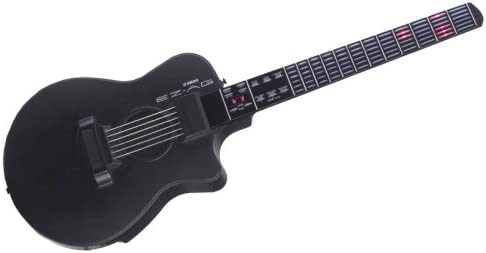
\includegraphics[scale=0.4]{Images/ezag.jpg}
%     \caption{The Yamaha EZ-AG is an \textit{instrument-like controller}.}
%     \label{fig:yamaha_wx7}
% \end{figure}

% There are a number of key motivating factors for this research, which arise from the constraints of traditional guitars, music information retrieval (MIR) based augmentation, and current guitar-based ILC up to this point.  

% The key motivations and themes of this work are outlined below.

% % =================================================
% \vspace{15pt}

% \begin{enumerate}
%     \item \textbf{Limitations of MIR based approaches}. Explain why MIDI pick ups aren't perfect, and why they may block creative flow, which is key to everything. How might MIR approaches work? Mention the traditional polyphonic approach or fret detection/resistance measurement. 
%     \item \textbf{Expanding the gestural palette for guitar-based ILC}. What are the drawbacks of ILDs like the Yamaha EZ-EG, and Starr Labs Explain why it could empower new kinds of expression for guitarists, which would be awesome. We want to support the tapping-style techniques which are demonstrated by MIDI guitar practitioners such as Rob Swire \cite{log_starr_2011} and Fabrizio Chiruzzi \cite{fabrizio_chiruzzi_channel_what_2010}.
%     \item \textbf{Guitar based MIDI control for composition professionals}. Explain why it would be useful to enable composers and producers to input musical data in a way which is most conducive to their muscle memory and creative flow. 
%     \item \textbf{Designing for true ambidextrous use}. Why is it important that products are able to support both right and left-handed users equally, and still be an appealing product to both, make sure you mention Norman \cite{norman_design_2013}.
%     \item \textbf{Inclusive design for limb-different users}. There has been generally very little support for guitarists with disabilities affecting the arms and upper body \cite{SOMETHING}, though, there has been great progress made by individual practitioners to develop techniques and technologies that support their creative vision. 
% \end{enumerate}



\section{Literature Review}
% \subsection{Research themes}

\subsection{The Augmented Guitar}
The NIME community has had a rich history of augmenting the guitar, among nearly all other instruments, to add new features. Recently, \cite{avila_augmenting_2019}, published a very comprehensive overview/framework for examining and conceiving new augmented guitar instruments. 

They observe that guitar augmentations are generally
vary across two dimensions, namely the degrees of \textit{invasiveness} and degrees of \textit{transformation}.

For example, \cite{martelloni_percussive_2020} experiment with a guitar augmentation that involved wrapping finger-style guitarist's acoustic guitars in bubble wrap, to examine how the new constraint had an impact on their creativity, and playing style. This would be an example of a \textit{low} invasiveness augmentation, since it can be easily done, and easily undone, with no permanent modification to the guitar. It arguably also has a low degree of transformation, since most of the essential properties and characteristics of the guitar remain the same. 

Another example is the GuitarAMI system which is put forth by \cite{meneses_guitarami_2018}, which involves adding sensors and pickups to a classical, nylon string guitar, which allow for extended gestures and sensors (tilt, accelerometer, cameras) to map to additional audio effects, for example reverb length/mix and sound reversal. This was controlled and processed by a digital foot-switch. This offers enormous scope for changing the sound of the instrument, but is non-permanent. Therefore, this augmentation has low invasiveness, but a high degree of transformation. 

An example of a guitar augmentation with high invasiveness might be that of adding a kill-switch to an electric guitar (a simple button connected to the guitar's inner circuit that disables the sound for the duration of the button press). This involves drilling a hole in the body of the guitar (a permanent change) and also soldering additional components and wires into the guitar's existing circuit, which is not impossible, but difficult to reverse. 

The proposed prototype falls into the extreme of both dimensions. As will be discussed in later sections this prototype falls into the extreme end of invasiveness with permanent drilling alterations into the neck of the guitar, but also with the removal of strings and replacement thereof with sensors, the degree of transformation is arguably quite high. 

Furthermore there have been more `smart' and network connected augmentations. \cite{turchet_ubiquitous_2019} have focused on creating a smart guitar for collaborative musical practice. This is immensely interesting since it offers the opportunity for a guitarist and a smartphone user to
practice music together using a smart guitar as a hub for
sound reproduction. 

Additionally, \cite{khalil_crowdsourced_2019} has developed a system for detecting note onsets and pitches using Music Information Retrieval (MIR) techniques which feeds an internet connected sampler, which will fetch audio samples based on the content of voice commands. For example, a user might speak "piano" into the smart guitar's in-built microphone and the on-board Bela will contact the  \href{https://freesound.org/}{\textbf{FreeSound}} API, and download an appropriate sample, and play it through the built-in sampler, in response to the user's guitar playing. 

Another approach was to implement deep learning in the augmentation of the guitar which is incredibly interesting. \cite{john_personalisation_2020} created a deep learning vision system to personalise the experience of the electric guitar, such that the computer vision system could recognise different individuals who were holding the guitar and swap effects chains and parameter values to match their preferences. 

\subsection{The guitar as an expressive MIDI Controller}

One might argue that the key theme in the rise of the guitar in modern culture, and perhaps the key to its success, has been innovation. Since 1932 \citep{millard_electric_2004} when the first electronically amplified guitar was introduced, practitioners and technologists have developed a plethora of technologies to electronically augment the capabilities of the guitar \citep{lahdeoja_approach_2008}. However since the dawn of MIDI in 1982 \citep{stubbs_mars_2018} the keyboard has become the standard for inputting MIDI information in modern studios, bedroom and professional alike \citep{roads_composing_2015}. This is a less-than-ideal situation, because this, to a certain extent, excludes certain types of musicians from being able to express their musical ideas in a way which is natural and intuitive for them, when composing computer music. This is problematic because there are approximately 7 million musicians in the United Kingdom\footnote{Based on there being 60 million people \citep{datacommons_united_2020} in the United Kingdom in 2006 (year of the BBC article) and 11.6\% of people in that year participating in playing a musical instrument.}, and 4 million of whom are guitarists \citep{bbc_uk_2006}. This means that there are up to 2 million people in the UK alone who are not supported by the traditional paradigm of keyboard MIDI controllers. This kind of discrepancy could be resolved by offering guitarists a viable alternative to using a keyboard to play in their musical ideas to the DAW. We further wish to prevent users from requiring to use a mouse to input musical data, since \cite{nash_supporting_2012} highlights how this practice can be highly antithetical to creative flow in the studio.

The current literature appears to be focused on the live performance of music. This presents an opportunity to focus on the \textit{studio} applications of the augmented guitar. MIDI keyboards have been popular in professional and home studios for many years, and with the rise of advanced, expressive MPE products like the ROLI Seaboard \citep{lamb_seaboard_2014}, guitarists have been left largely without an expressive controller which they can use in the studio to take advantage of the rich expressive world of MPE instruments. 

However, there have been a wide variety of very interesting and successful MIDI guitars in previous years. For example, the SynthAxe \citep{white_guitarists_1984} (see Figure \ref{fig:synthaxe}) is an incredibly comprehensive MIDI controller, offering strumming capabilities as well as buttons on the body which correspond to note activations. 

Though the product was not a commercial success, possibly as a result of its cost-prohibitive \$11,000 price \citep{metlay_musician-machine_1990}, there are several elements that contribute to this being a very expressive MIDI controller. The variety of supported playing styles is very wide, and therefore supports the creativity of users in as many ways as possible. The SynthAxe used `fret wiring' to detect the location of fingers on strings. For example, pressing the low E string on fret 1 would make a distinct circuit to the D string on fret 12, using this, gestures can be mapped into MIDI notes. It was also possible to bend the strings on the SynthAxe, which adds great expressive potential and leverages existing user expertise. However, \cite{metlay_musician-machine_1990} notes that despite its similarity to the traditional guitar, it ``required a fair amount of retraining to use properly". 

Furthermore, Roland Corporation have been offering commercially successful synthesizer augmentation for guitars for many years. For example the Roland GR-20 \citep{roland_roland_2021}. This involves a attaching a removable `divided pickup' (one sensor per string) to user's existing instruments, which then connects to a digital computer nested inside a stomp-box style interface. This again is an example of a low-invasiveness, high-transformation type augmentation. This allows users to use all their existing expert technique in controlling the new MIDI instrument, which is a highly desirable feature, and one which this prototype aims to achieve.  


\begin{figure}[h]
    \centering
    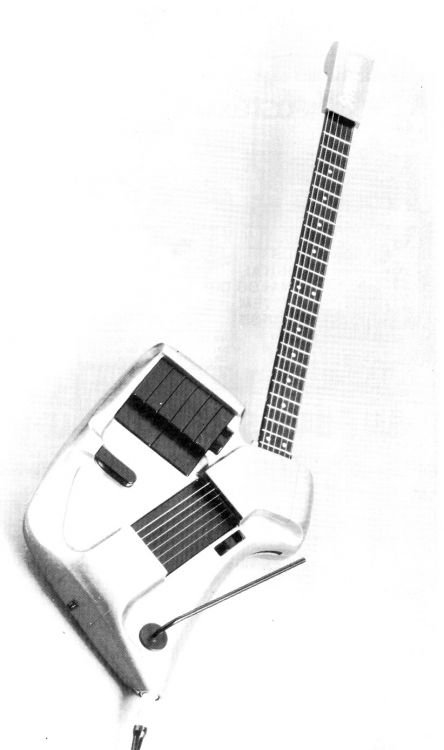
\includegraphics[scale=0.5]{Images/synthaxe.jpg}
    \caption{The \textit{SynthAxe}}
    \label{fig:synthaxe}
\end{figure}

The Yamaha EZ-EG \citep{yamaha_yamaha_2003} offers MIDI to the guitarist through the use of buttons. This is a good first step, but cannot offer aftertouch or pitch bends to the user, which limits its sonic capabilities. The Artihphon Instrument 1, is also making great steps in the right direction also incorporating elements of polyphonic aftertouch to the design, but cannot perform pitch bends on the neck of the guitar in the intuitive gesture that so many guitarists know and love. This project attempts to create a prototype that is not only capable of MPE pressure, but also of pitch bending. 



\subsection{Supporting Creativity and Flow in Studio Applications}
This study aims to develop the capacity of the augmented guitar to interact with digital instruments and DAWs in a musically pleasing and spontaneous way. As \cite{martelloni_percussive_2020} highlight, musicians can be wary of augmenting their performance with digital technologies, for fear of coming up short with respect to spontaneity and creativity.

This insight could either be framed in terms of how digital instruments are somehow inherently un-spontaneous and not conducive to supporting creativity; however, it could also be viewed as a design problem. This echoes the perspective of \cite{norman_design_2013}, where the burden of creating a compelling digital product is well within reach, but the burden to do so falls on the shoulders of the designer. Thus, the aim of the design is two-fold: to reduce the barriers to creativity that are experienced when interacting with technology, but also to further develop new and creatively useful ``contact points", developing on the research of \cite{lahdeoja_approach_2008}. Contact points are defined by \cite{lahdeoja_approach_2008} as a mapping of a physical gesture/object interaction with sound.

The way that we create music is becoming more digital and `in the box' \citep{nash_supporting_2012}. This means that the amount that musicians are interacting with their computers in a musical context is increasing, and therefore these perceived ``limitations" of digital technology need to be reduced. Since the technological capabilities of the computer are great, we might expect that it should also afford great creative opportunities. It would seem, however, that the limitation is in the \textit{design} of these new musical interfaces, not their technological prowess.


\section{Design}
\subsection{Prototype overview}
Instead of having physical strings strung between the head and the bridge of the guitar, we employ Bela Trill Bar sensors. These will be positioned across the frets which will provide pressure-sensitive multi-touch to the guitar. A basic outline of the prototype can be seen in Figure \ref{fig:proposed}. In this prototype, the strings have been completely removed, and we will only employ the sensor input. This is an experimental design, but is intended to work as a forcing function \citep{norman_design_2013} to encourage exploration of the novel MPE features. Furthermore, strings may impact on the accuracy of the sensor data. 

This design is akin to the Chapman Stick k\citep{stick_enterprises_stick_2021}, and encourages two hands on the frets as as shown in Figure \ref{fig:chapman}.

\begin{figure}[h]
    \centering
    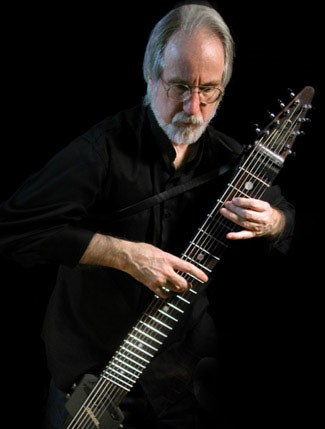
\includegraphics[scale=0.9]{Images/chapman.jpg}
    \caption{Chapman Stick style guitar, with a two-handed playing technique on the fretboard.}
    \label{fig:chapman}
\end{figure}

The prototype contains only six sensors in total, as any more is prohibitively expensive. The sensors occupy the 4th to 9th frets, as these are the frets which could accommodate the whole height of the Trill sensor. This means that on the frets which are occupied, all of the fret area is available to the user. 

The Bela Trill Bar sensors have a Grove connector on the back, so a small hole has been drilled through to neck to allow the wire to be passed through to the other side, so each sensor can be connected in series. Each of the sensors have also been trimmed to size to fit the appropriate width and height of their respective frets. 

With processing of the sensor data, this allows the array of sensors to act as if they were a matrix of fret-string locations, and thus can begin to emulate the behaviour of a traditional guitar.

Implementing the touch size and touch location data associated with each touch point will provide the data required to implement the MPE aftertouch and pitch bend functionality. 

The Bela Trill Bar sensors (Figure \ref{fig:trill_picture}) have been selected to play the central tole in this design for several reasons. Firstly, it affords multi-touch sensing, up to five simultaneous touches. which is sufficient for most guitar playing. 

It offers sensing in the horizontal direction only, but this is sufficient since notes are only differentiated horizontally on the guitar, and pitch bends (on traditional guitars) are also only available on this axis.

Secondly, it affords detection of touch size, which can be used as a proxy for pressure. Touch size and pressure are not the same, but are highly correlated. Therefore, we can use touch size in place of true pressure, and the prototype should offer a very similar behaviour compared to FSRs. In a more sophisticated prototype, we might consider incorporating additional sensors that can detect true pressure i.e. force sensitive resistors (FSRs). This would be beneficial as this would afford a more natural mapping between the gesture and the sound \citep{norman_design_2013}. This is because most acoustic instruments react to \textit{force} and not `touch size'. Therefore, a force-based interaction would represent an experience which is more representative of users experience with acoustic instruments which may be more successful overall. This is important as it links to \cite{norman_design_2013}'s 6th fundamental principal of design. Mapping in design, just like in mathematics, represents a connection between one set to another set. In this instance, the mapping of force exerted/touch size on the sensor, to the timbre (e.g. brightness) of the sound.  

\begin{figure}[h]
    \centering
    % 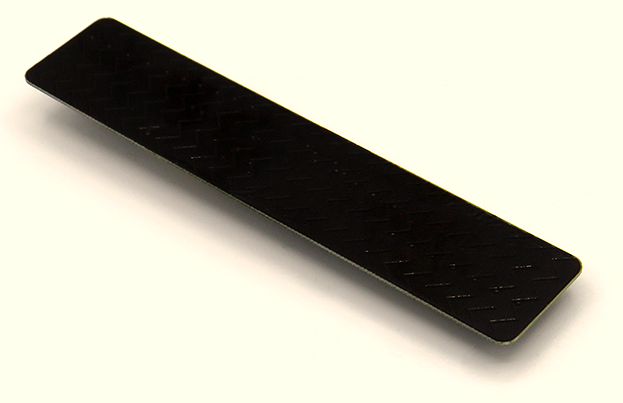
\includegraphics[scale=0.5]{Images/trill front.PNG}
    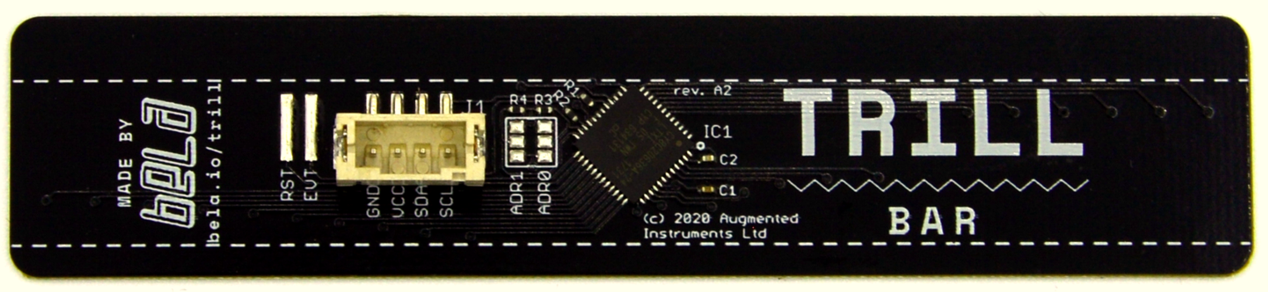
\includegraphics[scale=0.25]{Images/trill back.PNG}
    % \caption{Bela Trill Bar sensor front (top) and back (bottom). }
    \caption{Bela Trill Bar sensor. }
    \label{fig:trill_picture}
\end{figure}

In the design of this prototype, FSRs were also examined to be the principle sensor to comprise this design. As stated above, these do come with the added benefit of \textit{true} force sensing, not just using touch size as a proxy, which may result in a more expressive final product, but they also come with more drawbacks. 

However, this would only support pressure detection, and not pitch bending, since we would not be able to detect the continuous horizontal variance across the width of the frets which is essential for pitch bending. 

Furthermore, this would require a very large amount of analogue inputs into the micro-controller (one per fret-string location), which would rapidly be exhausted, as the number of frets supported increased. 

In future iterations of the design this could offer additional information on top of the capacitive sensors, which could make the instrument more expressive. 

\begin{figure}
    \centering
    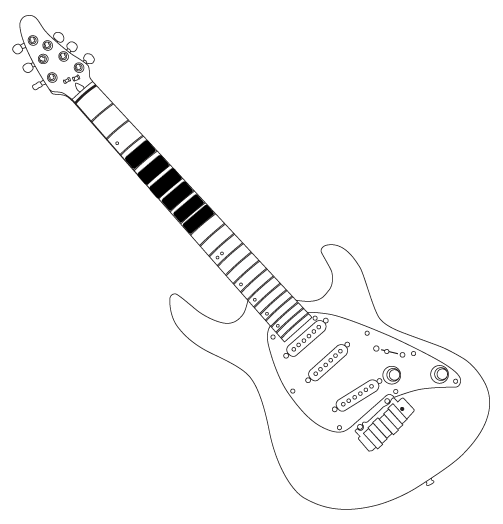
\includegraphics[scale=0.65]{Images/NEWGUITA.png}
    \caption{Basic prototype design}
    \label{fig:proposed}
\end{figure}

\begin{figure*}
    \centering
    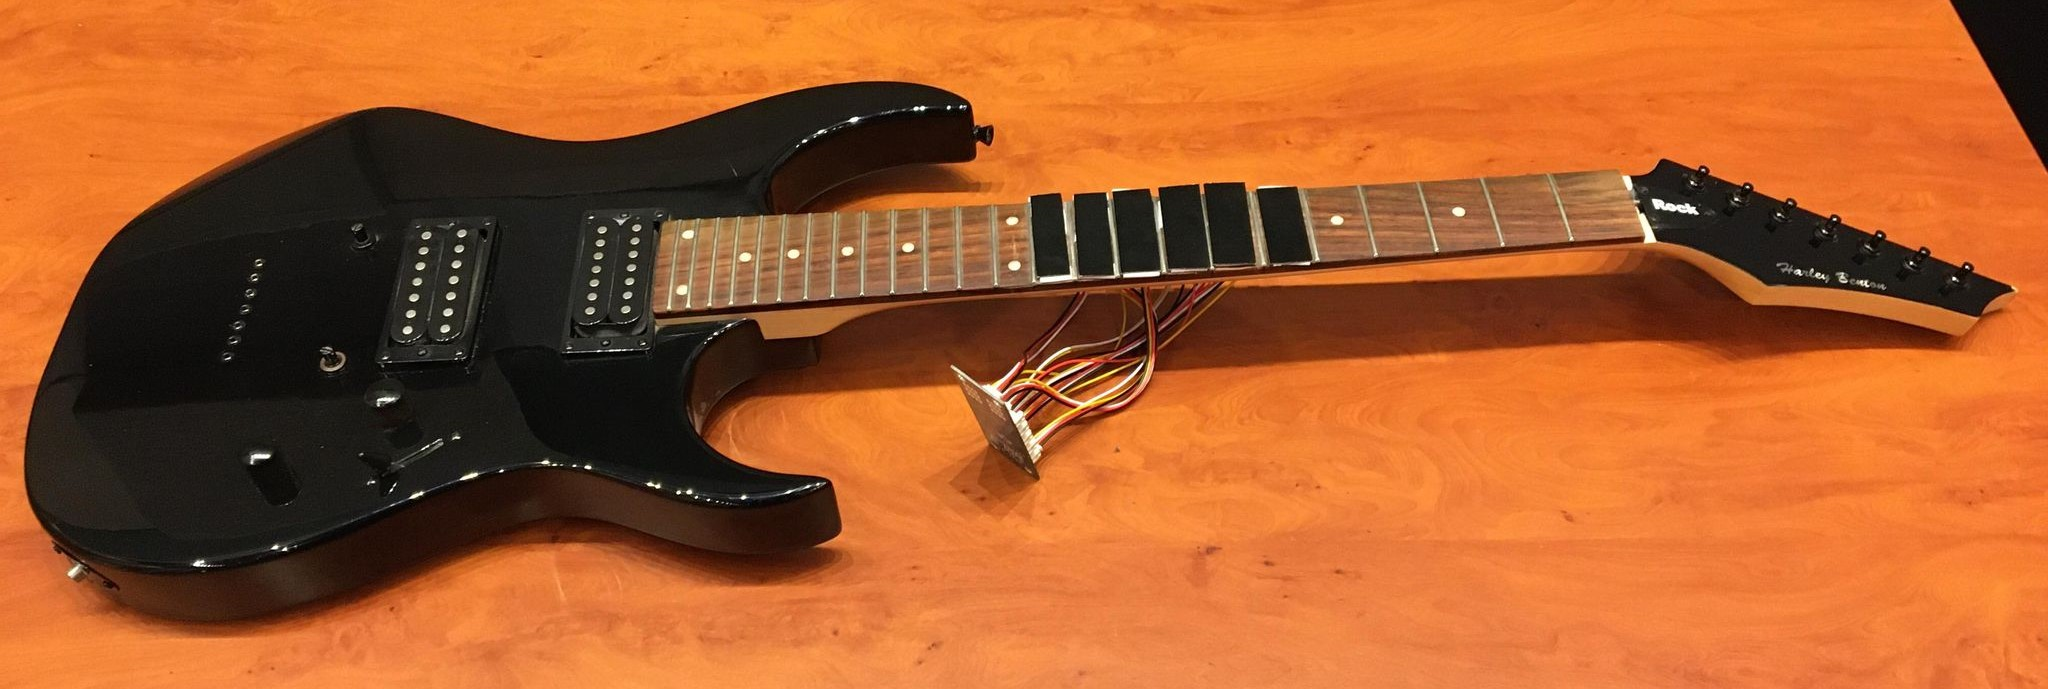
\includegraphics[scale=0.33]{Images/guitar1.jpg}
    \caption{Final prototype. See Appendix \ref{appendices:guitarimages} for more images of the final prototype.}
    \label{fig:guitarfront1}
\end{figure*}


% =========================================
\section{Software Implementation}

\subsection{Sensor to MIDI Translation}
We can summarise the logical overview of sensor input to MIDI instructions with the diagram shown in Figure \ref{fig:logicFlow}.
\subsubsection{Sensor discretisation \& touch identification}

\begin{figure}
    \centering
    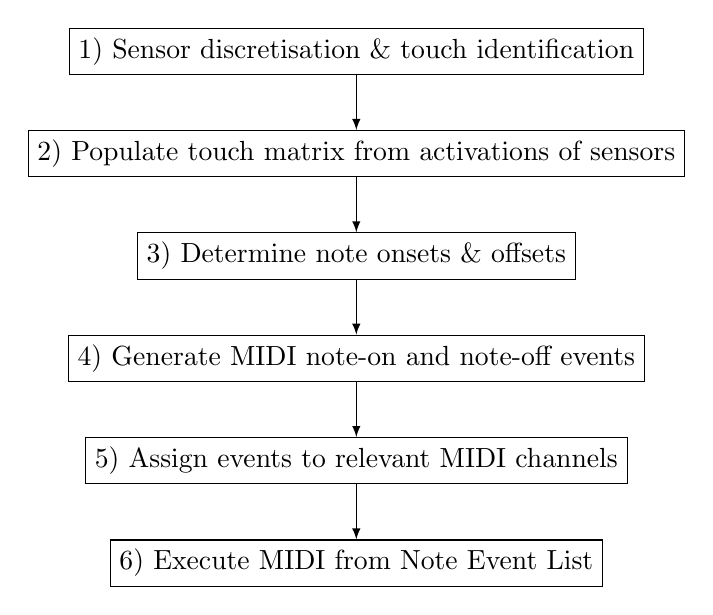
\begin{tikzpicture}
 [node distance=4.35cm]
\node (n1)[rectangle,draw]at (0,0) {1) Sensor discretisation \& touch identification};
\node (n2)[rectangle,draw] at ($(n1.south)+(0.0,-1.0)$) {2) Populate touch matrix from activations of sensors};
\node (n3)[rectangle,draw] at ($(n2.south)+(0.0,-1.0)$) {3) Determine note onsets \& offsets};
\node (n4)[rectangle,draw] at ($(n3.south)+(0.0,-1.0)$) {4) Generate MIDI note-on and note-off events};
\node (n5)[rectangle,draw] at ($(n4.south)+(0.0,-1.0)$) {5) Assign events to relevant MIDI channels};
\node (n6)[rectangle,draw] at ($(n5.south)+(0.0,-1.0)$) {6) Execute MIDI from Note Event List};

% Connectors
\draw [-latex] (n1) -- (n2);
\draw [-latex] (n2) -- (n3);
\draw [-latex] (n3) -- (n4);
\draw [-latex] (n4) -- (n5);
\draw [-latex] (n5) -- (n6);

\end{tikzpicture}
    \caption{Logical overview of the sensor data to MIDI event conversion.}
    \label{fig:logicFlow}
\end{figure}

Each fret of the system is represented by a Bela Trill Bar sensor, which has continuous expression in the horizontal axis.

We are then faced with the challenge of discretizing this continuous dimension into 'string zones', such that, if there are 6 strings (which is the case for the traditional guitar), all touches within the first sixth of the bar are categorized as string $0$, all touches within the second sixth of the bar are categorized as string $1$, and so on. 

Trill sensor data is already normalized to the range of $0$ to $1$, which means that the far 'left' of the sensor represents a mapping of $X$ to $0$, and the far right represents where $X$ maps to $1$.

Using this knowledge and knowing how many strings we want to use in the system we can determine the width and boundary locations of each string zone. Expression \ref{eq:string-boundaries} describes the set of string boundaries $\mathbf{B}$, which has length  $L$ and where $S$ is the number of strings.
\begin{equation} \label{eq:string-boundaries}
\mathbf{B}_n = \frac{n}{L}, \: \: \: \: \: \: \: \: n \in [0:S-1], \; \; \;  n \in \mathbb{Z}
\end{equation}

It is recognised that $S + 1$ boundaries are typically required to delineate a region completely, however, since we are bound to not receive input over $1.0$, this `implies' our final upper bound. We can use this fact to reduce the complexity of our program.

Having discretized all touches into string zones, and knowing their fret index, we can construct a binary matrix that represents touches on each fret-string location. This is required to determine note onset and offsets, which does not directly relate to the MPE behaviour of the system, but is a necessary pre-requisite for all MIDI instruments.


\newcommand{\trillWidth}{101.6mm / 1.2}
\newcommand{\trillHeight}{21.5mm / 1.2}
\newcommand{\NumStrings}{6}
\newcommand{\StringWidth}{\trillWidth/\NumStrings}
\begin{figure}[h]
    \centering
    \begin{tikzpicture}
    \usetikzlibrary{shapes.misc, positioning, svg.path}
    
    \fill [black,draw]
  {[rounded corners=6](0,0) --
  ++(\trillWidth, 0)  --
  ++(0, \trillHeight) --
  ++(-\trillWidth, 0) --
  cycle
  {}};

  \draw[white, thick, dashed] (0, 0) -- (0 ,\trillHeight);
  \draw[white, thick, dashed] (\StringWidth*1, 0) -- (\StringWidth*1 ,\trillHeight);
  \draw[white, thick, dashed] (\StringWidth*2, 0) -- (\StringWidth*2 ,\trillHeight);
  \draw[white, thick, dashed] (\StringWidth*3, 0) -- (\StringWidth*3 ,\trillHeight);
  \draw[white, thick, dashed] (\StringWidth*4, 0) -- (\StringWidth*4 ,\trillHeight);
  \draw[white, thick, dashed] (\StringWidth*5, 0) -- (\StringWidth*5 ,\trillHeight);
  
   %\draw[white, thick, dashed] (0, 0) -- (0 ,\trillHeight);
   \node[align=left] at (\StringWidth*0, -0.3) {0.0};
   \node[align=left] at (\StringWidth*1, -0.3) {0.16};
   \node[align=left] at (\StringWidth*2, -0.3) {0.33};
   \node[align=left] at (\StringWidth*3, -0.3) {0.50};
   \node[align=left] at (\StringWidth*4, -0.3) {0.66};
   \node[align=left] at (\StringWidth*5, -0.3) {0.83};
   
   \node[draw,circle, fill=red, text=white] at (\StringWidth/2 + \StringWidth*2,\trillHeight/2) {0.40};

    \end{tikzpicture}
    \caption{Demonstration of the sensor boundaries $\mathbf{B}_n$ for N=6. The vertical dashed lines represent the string boundaries $\mathbf{B}_n$, \textit{not} digital strings. }
    \label{fig:my_label}
\end{figure}

We can determine the string zone of the red dot with the following logic, shown is pseudo-code in Figure \ref{fig:getStringZone}. 
\begin{figure}[h]
    \centering
    \begin{verbatim}
int getStringZone(float touchLocation)
{
    for i=0:length(Bn):
        if(touchLocation >= Sn[i]):
            return i
    return -1 // Error, out of range. 
}
\end{verbatim}
    \caption{String zone determining algorithm pseudo-code.}
    \label{fig:getStringZone}
\end{figure}


Which will return $\mathbf{B}_n = 2$ for $S=6$. 

\subsubsection{Populate touch matrix from activations of sensors}
Since we know the index of each sensor, we can construct a strings $\times$ frets matrix like so. For example with three sensors, as is shown in Figure \ref{fig:trill_touches}, we can generate the binary matrix in Figure \ref{fig:binary_matrix}.

Here, we will also define the notation for discussing each individual cells of the matrix diagrams. In Figure \ref{fig:binary_matrix}, the $\mathbf{1}$ in the top row would have position $(0, 3)$, the middle row $(1, 0)$ and the bottom row $(2, 5)$. Fret index increases with vertical movement down, and string index increases with horizontal movement to the right. 


% \newcommand{\trillWidth}{101.6mm / 1.2}
% \newcommand{\trillHeight}{21.5mm / 1.2}
% \newcommand{\NumStrings}{6}
% \newcommand{\StringWidth}{\trillWidth/\NumStrings}
\begin{figure}[h]
    \centering
    \begin{tikzpicture}
    \usetikzlibrary{shapes.misc, positioning, svg.path}
    
    \fill [black,draw]
  {[rounded corners=6](0,0) --
  ++(\trillWidth, 0)  --
  ++(0, \trillHeight) --
  ++(-\trillWidth, 0) --
  cycle
  {}};
  \draw[white, thick, dashed] (0, 0) -- (0 ,\trillHeight);
  \draw[white, thick, dashed] (\StringWidth*1, 0) -- (\StringWidth*1 ,\trillHeight);
  \draw[white, thick, dashed] (\StringWidth*2, 0) -- (\StringWidth*2 ,\trillHeight);
  \draw[white, thick, dashed] (\StringWidth*3, 0) -- (\StringWidth*3 ,\trillHeight);
  \draw[white, thick, dashed] (\StringWidth*4, 0) -- (\StringWidth*4 ,\trillHeight);
  \draw[white, thick, dashed] (\StringWidth*5, 0) -- (\StringWidth*5 ,\trillHeight);
   
   \node[draw,circle, fill=red, text=white] at (\StringWidth/2 + \StringWidth*3,\trillHeight/2) {0.63};
    \end{tikzpicture}
    
     \centering
    \begin{tikzpicture}
    \usetikzlibrary{shapes.misc, positioning, svg.path}
    
    \fill [black,draw]
  {[rounded corners=6](0,0) --
  ++(\trillWidth, 0)  --
  ++(0, \trillHeight) --
  ++(-\trillWidth, 0) --
  cycle
  {}};
  \draw[white, thick, dashed] (0, 0) -- (0 ,\trillHeight);
  \draw[white, thick, dashed] (\StringWidth*1, 0) -- (\StringWidth*1 ,\trillHeight);
  \draw[white, thick, dashed] (\StringWidth*2, 0) -- (\StringWidth*2 ,\trillHeight);
  \draw[white, thick, dashed] (\StringWidth*3, 0) -- (\StringWidth*3 ,\trillHeight);
  \draw[white, thick, dashed] (\StringWidth*4, 0) -- (\StringWidth*4 ,\trillHeight);
  \draw[white, thick, dashed] (\StringWidth*5, 0) -- (\StringWidth*5 ,\trillHeight);
   
   \node[draw,circle, fill=red, text=white] at (\StringWidth/2 + \StringWidth*0,\trillHeight/2) {0.08};
   
    \end{tikzpicture}
    
     \centering
    \begin{tikzpicture}
    \usetikzlibrary{shapes.misc, positioning, svg.path}
    
    \fill [black,draw]
  {[rounded corners=6](0,0) --
  ++(\trillWidth, 0)  --
  ++(0, \trillHeight) --
  ++(-\trillWidth, 0) --
  cycle
  {}};
  \draw[white, thick, dashed] (0, 0) -- (0 ,\trillHeight);
  \draw[white, thick, dashed] (\StringWidth*1, 0) -- (\StringWidth*1 ,\trillHeight);
  \draw[white, thick, dashed] (\StringWidth*2, 0) -- (\StringWidth*2 ,\trillHeight);
  \draw[white, thick, dashed] (\StringWidth*3, 0) -- (\StringWidth*3 ,\trillHeight);
  \draw[white, thick, dashed] (\StringWidth*4, 0) -- (\StringWidth*4 ,\trillHeight);
  \draw[white, thick, dashed] (\StringWidth*5, 0) -- (\StringWidth*5 ,\trillHeight);
   
   \node[draw,circle, fill=red, text=white] at (\StringWidth/2 + \StringWidth*5,\trillHeight/2) {0.91};
   
    \end{tikzpicture}
    
    \caption{Example of sensors with touch locations in the relevant string zones. The vertical dashed lines represent the string boundaries $\mathbf{B}_n$, \textit{not} digital strings. }
    \label{fig:trill_touches}
\end{figure}

\begin{figure}[h]
    \centering
    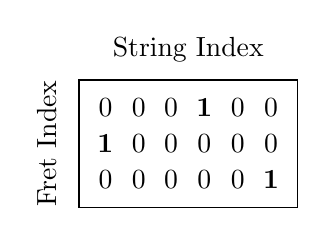
\begin{tikzpicture}
    \matrix (mD) [draw,matrix of math nodes]
    {
    0 & 0 & 0 & \textbf{1} & 0 & 0 \\
    \textbf{1} & 0 & 0 & 0 & 0 & 0 \\
    0 & 0 & 0 & 0 & 0 & \textbf{1} \\
    };
    
    \node[rotate=90] at (-1.8cm, 0) {Fret Index};
    \node at (-0.0cm, 1.2cm) {String Index};
    
    \end{tikzpicture}
    \caption{Binary matrix interpreted from sensor positions.}
    \label{fig:binary_matrix}
\end{figure}

\subsubsection{Determine note onsets \& offsets}
Note-on and note-off events are not trivial to detect as they can only be determined \textit{between} audio callbacks, not \textit{within}. Meaning, that no single `snapshot' of a touch matrix is sufficient to determine note onsets or offsets. This means that there must be a system for `remembering' which fret-string locations were active in the previous audio callbacks. 

This is achieved by the comparison of a \textit{pair} of binary matrices,  where each element represents a logical Boolean value. One matrix, $\mathbf{C}$, represents the \textbf{c}urrent activation (presence of touch) of fret-string locations in the audio callback and one matrix, $\mathbf{P}$, which represents activations in the \textbf{p}revious audio callback.

To determine note onsets, we can perform the following element-wise logical operation on $\mathbf{C}$ and $\mathbf{P}$, which will generate a third binary matrix,  $\mathbf{Onsets}$, which represents the position of note onsets. 
\begin{equation} \label{eq:onsets}
\begin{aligned}
\mathbf{Onsets}_{f,s} := \mathbf{C}_{f,s} \land \lnot \mathbf{P}_{f,s}, \\
 f \in [0:F-1],  \: \:  s \in [0:S-1]
\end{aligned}
\end{equation}

Where $F$ is the number of `frets' and $S$ is the number of `strings'. 

What follows is the matching expression for the note off binary matrix, $\mathbf{Offsets}$. 

\begin{equation} \label{eq:offsets}
\begin{aligned}
\mathbf{Offsets}_{f,s} := \lnot \mathbf{C}_{f,s} \land \mathbf{P}_{f,s}, \\
 f \in [0:F-1],  \: \:  s \in [0:S-1]
\end{aligned}
\end{equation}

This is visually expressed with a simplified example in Figure \ref{fig:fret-matrix}.
\begin{figure}[h]
\centering
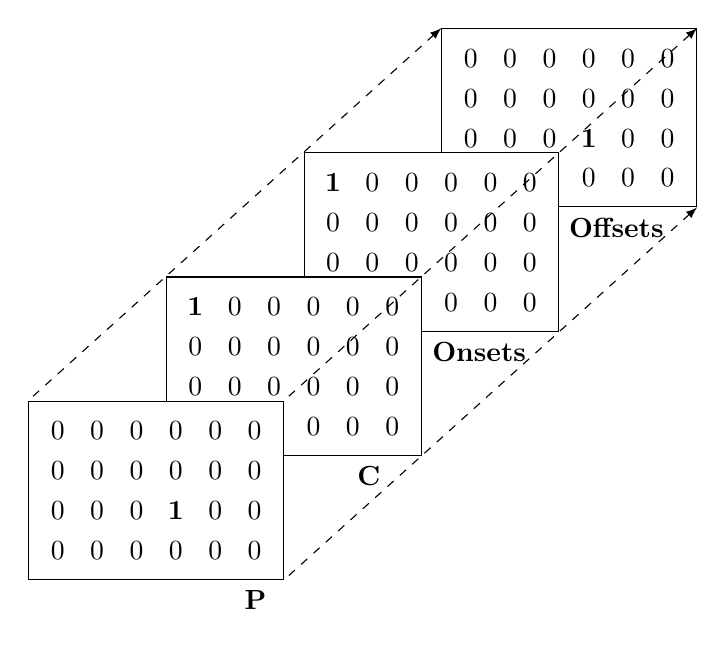
\begin{tikzpicture}[every node/.style={anchor=north east, fill=white, minimum width=0.5cm, minimum height=5mm}]

% OFFSETS
\matrix (mA) [draw,matrix of math nodes]
{
0 & 0 & 0 & 0 & 0 & 0 \\
0 & 0 & 0 & 0 & 0 & 0 \\
0 & 0 & 0 & \mathbf{1} & 0 & 0 \\
0 & 0 & 0 & 0 & 0 & 0 \\
};

% ONSETS
\matrix (mB) [draw,matrix of math nodes] at ($(mA.south west)+(1.5,0.7)$)
{
\mathbf{1} & 0 & 0 & 0 & 0 & 0 \\
0 & 0 & 0 & 0 & 0 & 0 \\
0 & 0 & 0 & 0 & 0 & 0 \\
0 & 0 & 0 & 0 & 0 & 0 \\
};

% C
\matrix (mC) [draw,matrix of math nodes] at ($(mB.south west)+(1.5,0.7)$)
{
\mathbf{1} & 0 & 0 & 0 & 0 & 0 \\
0 & 0 & 0 & 0 & 0 & 0 \\
0 & 0 & 0 & 0 & 0 & 0 \\
0 & 0 & 0 & 0 & 0 & 0 \\
};

% P
\matrix (mD) [draw,matrix of math nodes] at ($(mC.south west)+(1.5,0.7)$)
{
0 & 0 & 0 & 0 & 0 & 0 \\
0 & 0 & 0 & 0 & 0 & 0 \\
0 & 0 & 0 & \mathbf{1} & 0 & 0 \\
0 & 0 & 0 & 0 & 0 & 0 \\
};

\node[align=left] at ($(mD.south east) + (-0.1cm, -0cm)$){$\mathbf{P}$};
\node[align=left] at ($(mC.south east) + (-0.4cm, -0cm)$) {$\mathbf{C}$};
\node[align=left] at ($(mB.south east) + (-0.3cm, -0cm)$) {$\mathbf{Onsets}$};
\node[align=left] at ($(mA.south east) + (-0.3cm, -0cm)$) {$\mathbf{Offsets}$};

\draw[latex-, dashed](mA.north east)--(mD.north east);
\draw[latex-, dashed](mA.north west)--(mD.north west);
\draw[latex-, dashed](mA.south east)--(mD.south east);
\end{tikzpicture}

\caption{Demonstration of binary matrix operation for onsets and offsets using the expressions \ref{eq:onsets} and \ref{eq:offsets}}
\label{fig:fret-matrix}

\end{figure}

\subsubsection{Generate MIDI note-on and note-off events}

At this point it is possible to convert fret-string locations to MIDI number, and send the required MIDI note-on and note-off instructions. However, this presents us with a problem that is unique to guitar-style MIDI controllers.

We must convert the $\mathbf{Onsets}$ and $\mathbf{Offsets}$ into MIDI instructions so that our prototype can communicate with digital instruments and DAWs in a format that is understood.

Furthermore, we must `remember' which notes are currently \textit{active} (have had an onset, but hasn't yet had an offset), and to ensure that all \textit{active} notes are correctly terminated at the appropriate time. Failing to do this will result in notes that do not correctly stop at the right time, creating a cacophonous barrage of notes which will ultimately be frustrating for the user.

This requires that each fret-string location is individually addressable, such that when location $(0, 1)$ has an onset corresponding to MIDI note $45$, for example, when that corresponding offset is sent, that note is in fact terminated.

We might be tempted to use MIDI notes as the identifier for fret-string locations such that when $(0, 1)$ is played we store in memory that note $45$ is currently active, and when we receive the corresponding offset that matches up with MIDI note $45$, we terminate that note. This logic would work fine for a piano or keyboard MIDI controller, because each key has a \textit{unique} mapping to any given MIDI note. This is not the case with the guitar. Figure \ref{fig:midicantormatrix}a shows the mapping of fret-string locations to MIDI note number for standard EADGBE guitar tuning.

\newcommand{\higl}[1]{\textit{\textbf{#1}}}
\begin{figure}[h]
    \centering
    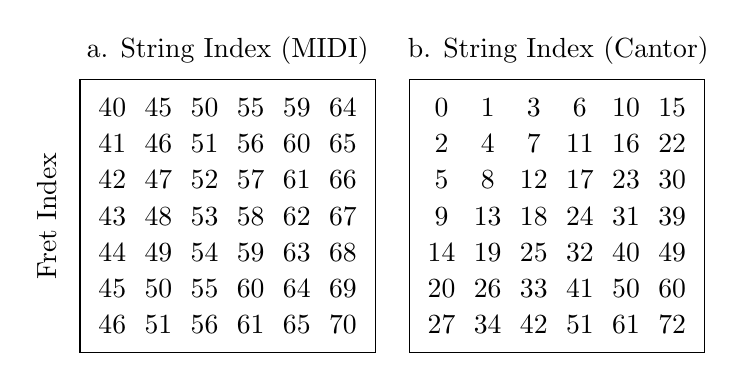
\begin{tikzpicture}
    \matrix (midi) [draw,matrix of math nodes]
    {
    40 & \higl{45} & \higl{50} & \higl{55} & \higl{59} & \higl{64} \\
    41 & \higl{46} & \higl{51} & \higl{56} & \higl{60} & \higl{65} \\
    42 & 47 & 52 & 57 & 61 & 66 \\
    43 & 48 & 53 & 58 & 62 & 67 \\
    44 & 49 & 54 & 59 & 63 & 68 \\
    \higl{45} & \higl{50} & \higl{55} & \higl{60} & \higl{64} & 69 \\
    \higl{46} & \higl{51} & \higl{56} & \higl{61} & \higl{65} & 70 \\
    };
    
    \matrix (cantor) [draw,matrix of math nodes] at ($(midi.east)+(2.3, 0.0)$)
    {
    0&	1&	3&	6&	10&	15& \\
    2&	4&	7&	11&	16&	22&\\
    5&	8&	12&	17&	23&	30&\\
    9&	13&	18&	24&	31&	39&\\
    14&	19&	25&	32&	40&	49&\\
    20&	26&	33&	41&	50&	60&\\
    27&	34&	42&	51&	61&	72&\\
    };
    
    \node[rotate=90] at (-2.3cm, 0) {Fret Index};
    \node at (-0.0cm, 2.1cm) {a. String Index (MIDI)};
    \node at (4.2cm, 2.1cm)  {b. String Index (Cantor)};
    
    \end{tikzpicture}
    \caption{Demonstration that there are not unique mappings from fret-string locations to MIDI notes, which therefore cannot be used as unique identifiers for notes. Highlighted numbers are non-unique. Diagram represent the first seven frets. }
    \label{fig:midicantormatrix}
\end{figure}

It can clearly be seen that there are MIDI note duplicates in this matrix, which means that there is not a unique mapping of fret-string locations to MIDI notes. This means that a user might press $(0, 1)$ for example, and then presses $(5, 0)$, this would override the former, and both notes would be terminated if either touch were released. 

This behaviour is not analogous to any typical acoustic instrument, and is therefore unlikely to match up with user's expectations. This unexpected behaviour is not only likely to disturb the user's workflow, but is also limits the possible actions of the user, which may not be conducive to their creativity.

% This behaviour is unlikely to match up with user's expectations in an unpleasing way, as they would expect independent behaviour for notes. 

Therefore, we require another method for uniquely identifying fret-string locations. For this we can use the Cantor pairing algorithm. This expression creates an ordered mapping between all pairs of natural numbers to the set of natural numbers. The expression for a two-element Cantor pairing is defined as so:

\begin{equation} \label{eq:cantor}
    \pi(k_1, k_2) := \frac{1}{2}(k_1 + k_2)(k_1 + k_2 + 1) + k_2
\end{equation}


\tikzset{->-/.style={decoration={
  markings,
  mark=at position #1 with {\arrow{>}}},postaction={decorate}}}
  
\begin{figure}[h]
    \centering
    
    \begin{tikzpicture}[scale=2.2]
    \clip(-0.60,-0.60) rectangle (3.40,3.45);
    \tkzInit[xmax=4,ymax=4,xmin=0,ymin=0]
    \tkzGrid
    \tkzAxeXY
    \node at (1.75, -0.5){\large $k_1$};
    \node[] at (-0.5, 1.75){\large $k_2$};
    
    % Draws the first blue line and red circle.
    \draw[thick,->-=.5,blue] (0,0) -- (1,0);
    \filldraw (0,0)[red] circle (1.7pt);
    
    % <THIS DRAWS THE BLUE LINES>
    \newcounter{N}{0}
    \foreach \n in {1,...,15} {
        \foreach \i in {0,...,\value{N}}{
            \draw[thick, ->-=.5,blue] (\n - \i, \i) -- (\n - 1 - \i ,\i + 1);
        }
        \stepcounter{N}
        \draw[thick, ->-=.5,blue] (0,\n) -- (\n+1,0); %IMPORTANT
    } % END <THIS DRAWS THE BLUE LINES>
    
    % <THIS DRAWS THE NUMBER AND RED DOTS>
    % These are 'registers' used to calculate the cantor number. 
    \setcounter{N}{3}
    \newcounter{cn}{0}
    \newcounter{r1}{0}
    \newcounter{r2}{0}
    \newcounter{r3}{0}
    \foreach \n in {0,...,3} {
        \foreach \i in {0,...,\value{N}}{
            % Fill circles. 
            \filldraw (\i, \n)[red] circle (1.5pt);
            
            %% CALCULATE CANTOR NUMBER
            % Reset registers. 
            \setcounter{cn}{0}
            \setcounter{r1}{\i}
            \setcounter{r2}{\n}
            \setcounter{r3}{0}
            
            % cn = (k1 + k2 + 1)
            \addtocounter{cn}{\value{r1}}
            \addtocounter{cn}{\value{r2}}
            \addtocounter{cn}{1}
            
            % r3 = (k1 + k2)
            \addtocounter{r3}{\value{r1}}
            \addtocounter{r3}{\value{r2}}
            
            % cn *= r3
            \multiply\value{cn} by \value{r3}
            
            % cn /= 2
            \divide\value{cn} by 2
            
            % cn += k2
            \addtocounter{cn}{\value{r2}}
            %% END CALCULATE CANTOR NUMBER
            
            % Display cantor number. 
            \node at (\i + 0.125, \n + 0.125){\arabic{cn}};
        }
    } % END <THIS DRAWS THE NUMBERS AND RED DOTS>
   
\end{tikzpicture}
    \caption{Visualization of the two element Cantor pairing algorithm.}
    \label{fig:my_label}
\end{figure}



Which means that each fret-string location can now be uniquely identified by a single integer. This means that we can now easily distinguish note events which have identical MIDI note values. We can compare the identifier numbers for each fret-string location by looking at Figure \ref{fig:midicantormatrix}. Note that in Figure \ref{fig:midicantormatrix}b that there is no duplication in any of the cells of the matrix. 

\subsubsection{Assign events to relevant MIDI channels}
Furthermore, to create MPE behaviour, we must be able to assign notes uniquely to MIDI channels in an efficient way. The MIDI 1.0 Protocol works in such a way that each MIDI \textit{channel} has pitch-bend and aftertouch, not each \textit{note}. This means that every note on any given channel would all be equally detuned by the same pitch bend instruction. This is typically very unmusical because very few acoustic instruments exhibit behaviour like this. 

This is the motivation to implement MPE behaviour, where each note is assigned to its own channel and thus had independent pitch-bend and after-touch, making for a more expressive instrument. 

However this represents a more complex programming task in both the controller/sensor design and the software instrument design. 
We must remember which notes, or indeed fret-string hashes as determined by expression \ref{eq:cantor}, are currently active. Furthermore, we must free MIDI channels as notes receive their offsets, such that we always choose the lowest index MIDI channel as possible. There are only 16 in total, and wish to avoid sending an invalid MIDI instructions, which may crash either one of the controller or MIDI host, which will prevent the user from working.

To complete this task we can create a length 16 list of `active notes'. Which represents the maximum number of MIDI channels and the maximum number of possible simultaneous notes playable on this controller. This limit is very likely to be sufficient, a maximum of 6 notes are expected (one per string) and a theoretical maximum of 10 notes are playable (one per finger), though the latter would represent a rather experimental technique. 

To create the behaviour required, we require multiple data points about each note event, and thus the list (implemented with a C++ standard library \texttt{vector}) is populated with the data structure shown in Figure \ref{fig:noteevent}.
\begin{figure}[h]
\begin{mdframed}
    \begin{verbnobox}[\small]
struct NoteEvent
{
    	int midiNote = -1;
    	int midiChannel = -1;
    	int velocity = -1;
    	int pressure = -1;
    	int pitchBend = -1;
    	float initialTouchLocation = -1;
    	int fretStringHash = -1;
    	bool isActive = false;
    	bool dueOnset  = false;
    	bool dueOffset = false;
};
    \end{verbnobox}
    \end{mdframed}
        \caption{\texttt{NoteEvent} data structure.}
    \label{fig:noteevent}
\end{figure}

In this data structure there are some other elements which will be discussed in later sections about MIDI continuous control (CC) instructions.

We can use this list of \texttt{NoteEvents} in order to describe which note events should be executed.

When a new note onset is detected, we can determine which element in the list it should occupy with the algorithm described in Figure \ref{fig:noteon}. This algorithm ensures that the selected index in the \texttt{noteEventList} is as small as possible. 

\begin{figure}[H]
\begin{mdframed}
\begin{verbnobox}[\small]
let noteEventList = vector<NoteEvent>{16}
let newOnset = {fret, str, ...}

for i=0:length(noteEventData)-1:
{
    if(!noteEventData[i].isActive)
    {
         noteEventData[i] = newOnset
         noteEventData[i].dueOnset = true
         noteEventData[i].isActive = true
    }
}
\end{verbnobox}
\end{mdframed}
\caption{Pseudo-code algorithm for determining the index of and creating new \texttt{NoteEvent} objects.}
\label{fig:noteon}
\end{figure}

Conversely, when a note offset is detected, and stated in the $\mathbf{Offsets}$ matrix, we can perform the following algorithm to edit the \texttt{noteEventList}.


\begin{figure}[h]
\begin{mdframed}
\begin{verbnobox}[\small]
let noteEventList = vector<NoteEvent>{16}
let newOnset = {fret, str, ...}

for i=0:length(midiList)-1:
{
    if(noteList[i].fsHash==cPair(fret,str))
    {
         noteList[i].isDueNoteOffset = true
    }
}
\end{verbnobox}
    \end{mdframed}
        \caption{Pseudo-code to mark \texttt{NoteEvent}s as ready to recieve a MIDI note off event.}
    \label{fig:noteoff}
\end{figure}

Conveniently, we can use the indices of the \texttt{NoteEvent} list to determine the MIDI channel for each note, as they are always the lowest value possible for a given note, and unique to each note. This is the case because as we can see in line 5 of Figure \ref{fig:noteon} as we iterate over \texttt{i}, we will `stop' at the lowest value of \texttt{i} that does not contain an active note and assign it the new note. 

\subsubsection{Execute MIDI from Note Event List}
Now we have a list of which MIDI notes to turn on and off, appropriately matched to a channel such that we can take advantage of MPE style behaviour.

This can be done by the C++ function in Figure \ref{fig:write_midi_function}, which implements the Bela MIDI API.

\begin{figure}[h]
\begin{mdframed}
\begin{lstlisting}
#define CH0_NOTE_ON  144
#define CH0_NOTE_OFF 128
using Midi = midi_byte_t;
void writeNote(int event, // 0->ON, 1->OFF
               int ch,    // midi channel
               Midi note, // note number
               Midi vel = 0) // velocity 
{
    int eventType = (event == 0)
            ? CH0_NOTE_ON : CH0_NOTE_OFF;
    Midi status =  Midi(eventType + ch);
    Midi out[3] = {status, note, vel};
    midi.writeOutput(out, 3);
}
\end{lstlisting}
\end{mdframed}
        \caption{C++ code using the Bela MIDI API to send note-on and note-off instructions.}
    \label{fig:noteoff}
\end{figure}

We then need to iterate though all elements of \texttt{NoteEvent}s and perform the proper function, which can be implemented with the code outlined in Figure \ref{fig:write_midi_function}.

\begin{figure*}[h]
\begin{mdframed}
\begin{lstlisting}
void writeMidiFromNoteEvents()
{
    for(int i = 0; i < gNoteEventData.size(); i++)
    {
        if(gNoteEventData[i].isActive)
        {
            if(gNoteEventData[i].isDueNoteOffset)
            {
                writeNote(1, i, gNoteEventData[i].midiNote);
                gNoteEventData[i].isDueNoteOffset = false;
                gNoteEventData[i].isActive = false;
            }
			
            if(gNoteEventData[i].isDueNoteOnset)
            {
                gNoteEventData[i].isDueNoteOnset = false;
                writeNote(0, i, gNoteEventData[i].midiNote, gNoteEventData[i].velocity);
            }
				
            writeAftertouch(i, gNoteEventData[i].pressure);
            midi.writePitchBend((midi_byte_t)i, gNoteEventData[i].pitchBend);
        }
    }
}
\end{lstlisting}
\end{mdframed}
    \caption{C++ code using the Bela MIDI API to send note-on and note-off instructions.}
    \label{fig:write_midi_function}
\end{figure*}

%TODO FINISH THIS SECTION

\subsection{MPE Aftertouch and Pitchbend}

Currently, we have only discussed how to implement basic note onsets and note offsets. While necessary, this is not sufficient to meet our requirement to implement MPE style behaviour. In order to create a compelling MPE experience, it is typical to implement aftertouch and pitch bend functionality. 

\textbf{Aftertouch} typically is an expression of `pressure' which can be expressed \textit{after} the onset of the note. It is typically used to map a force/pressure on a key to a note's amplitude or timbre. This might be likened to a saxophonist who may start a note by breathing quietly, and then crescendo the amplitude of the note before its offset. As stated above, force from an FSR would possibly make a more appropriate input for this parameter, however we are limited by the capabilities of the Bela Trill sensors, which can only interpret touch size. However, this does serve as a very reasonable proxy for force/pressure.

Since the acoustic and electric guitar is a plucked/strummed instrument, this type of expression is typically not available. This attempt to extend the expressive capacity of the guitar or guitar-like instruments is central to the motivation of this study.

\textbf{Pitchbend} is a feature which is typically implemented by a wheel to the left of the keys on standard MIDI keyboards (see Figure \ref{fig:pitchwheel}).

\begin{figure}[h]
    \centering
    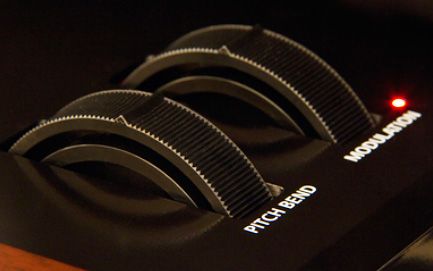
\includegraphics[scale=0.5]{Images/pitch bend.jpg}
    \caption{Typical pitch bend wheel}
    \label{fig:pitchwheel}
\end{figure}

However since we would like to emulate the expressive bending of guitar strings with this design, we must convert the touch location data into meaningful MIDI pitchbend data.s

These features can be implemented by a simple extension of the framework laid out above. In our basic touch matrices shown in Figures \ref{fig:binary_matrix} and \ref{fig:fret-matrix}, we store only a single Boolean value. Instead, we could store a more complex data structure which will help implement our MPE behaviour based on other sensor data such touch size and touch location. 

For each touch on each sensor, we must collect three important pieces of information. 

\begin{itemize}
    \item \texttt{bool isActive}: Whether this location in the fret-string matrix currently has a touch present.
    \item \texttt{float touchSize}: The size of the touch. This is a proxy for pressure, and can be used to implement our aftertouch functionality. 
    \item \texttt{float touchLocation}: The precise location on the sensor where the touch currently is.  
\end{itemize}

Now, each matrix $\mathbf{C}$ and $\mathbf{P}$ can be considered a 3D data structure, which would represent the arrangement of touches shown in Figure \ref{fig:trill_touches} in the following diagram, Figure \ref{fig:new_struct}. This assumes all touch sizes are 0.5 for simplicity, however this is entirely variable between 0 and 1. 

\begin{figure}[h]
\centering
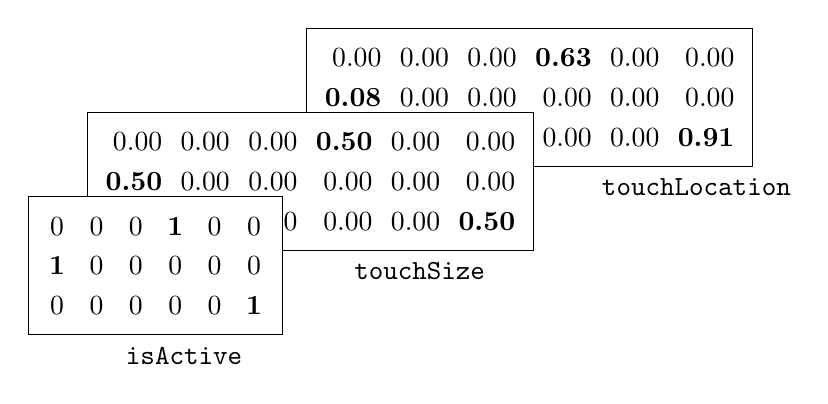
\begin{tikzpicture}[every node/.style={anchor=north east, fill=white, minimum width=0.5cm, minimum height=5mm}]



% OFFSETS
\matrix (mA) [draw,matrix of math nodes]
{
0.00 & 0.00 & 0.00 & \textbf{0.63} & 0.00 & 0.00 \\
\textbf{0.08} & 0.00 & 0.00 & 0.00 & 0.00 & 0.00 \\
0.00 & 0.00 & 0.00 & 0.00 & 0.00 & \textbf{0.91} \\
};

% ONSETS
\matrix (mB) [draw,matrix of math nodes] at ($(mA.south west)+(2.9,0.7)$)
{
0.00 & 0.00 & 0.00 & \textbf{0.50} & 0.00 & 0.00 \\
\textbf{0.50} & 0.00 & 0.00 & 0.00 & 0.00 & 0.00 \\
0.00 & 0.00 & 0.00 & 0.00 & 0.00 & \textbf{0.50} \\
};

% C
\matrix (mC) [draw,matrix of math nodes] at ($(mB.south west)+(2.5,0.7)$)
{
0 & 0 & 0 & \textbf{1} & 0 & 0 \\
\textbf{1} & 0 & 0 & 0 & 0 & 0 \\
0 & 0 & 0 & 0 & 0 & \textbf{1} \\
};

\node[align=left] at ($(mC.south east) + (-0.4cm, -0cm)$) {\texttt{isActive}};
\node[align=left] at ($(mB.south east) + (-0.5cm, -0cm)$) {\texttt{touchSize}};
\node[align=left] at ($(mA.south east) + (0.6cm, -0cm)$) {\texttt{touchLocation}};
\end{tikzpicture}

\caption{A visual representation of the updated data structure used to represent touch information. }
\label{fig:new_struct}

\end{figure}
 
In the case of aftertouch, all that must be done is to look up the fret-string/Cantor hash of the given location, scale the touch size to the given aftertouch range as specified by the MIDI 1.0 documentation, and write the result to the output as per Figure \ref{fig:write_midi_function}. This scaling can be achieved by the following means:

\DeclarePairedDelimiter\ceil{\lceil}{\rceil}
\DeclarePairedDelimiter\floor{\lfloor}{\rfloor}
\begin{equation}
    y = \floor{x \cdot AT_{max}}
    \label{eq:scaling}
\end{equation}

Where $AT_{max}$ is the maximum valid aftertouch value. This expression can also be used with maximum velocity $V_{max}$ to give meaningful and valid velocity readings. From the Bela Trill API and touch location and touch size are already normalized to between 0 and 1. 

Implementing pitch bend behaviour in this application requires more creative decisions to be made, as there is not a predefined or standard implementation. 

On a typical electric or acoustic guitar, pitch bending is achieved by the physical \textit{bending} of the string which causes the tension of the string to increase, which results in the string oscillating at a higher frequency. 

In the case of this prototype, we do not have strings at all, only the \texttt{touchLocation} data point per note. 

In this prototype we have chosen to implement the feature like so. 

\begin{enumerate}
    \item When a note is onset, start the pitchbend amount at zero, regardless of the \texttt{touchLocation}. 
    \item Make a note of the initial \texttt{touchLocation}. 
    \item On each subsequent audio callback, we can subtract the initial \texttt{touchLocation}, with the current  \texttt{touchLocation}, and scale that to within the valid MIDI pitch bend range. 
\end{enumerate}

This behaviour was chosen since, this is a new instrument, defining pitch bend absolutely with respect to touch position within each string region would require users to have very exact positioning on the sensor. Failure to do this would result in out of tune notes. 

The implemented behaviour only requires that users touch the right string zone, and they do not have to worry about tuning. They can just bend from wherever they land their finger in the touch zone, which should make for a more pleasurable playing experience. 

To create the mapping from the difference between the initial \texttt{touchLocation}, and the present one to calculate the pitchbend amount took some experimentation, but the expression is shown below in expression \ref{eq:pitchbend}:

\begin{equation}
    PB = 2 \cdot PB_{max} \left( \frac{T_i-T_c}{\Delta T_{max}} \right)^\alpha - \frac{PB_{max}}{2}
    \label{eq:pitchbend}
\end{equation}

Where $PB_{max}$ is the maximum pitch bend value of 16383; $T_i$ and $T_c$ are the intial and current touch locations respectively and $\Delta T_{max}$ is the maximum difference between $T_c$ and $T_i$ (i.e. the width of a given string region).

The maximum pitch bend value refers to the maximum numerical value that is accepted in the MIDI 1.0 specification. 16383 maps to maximum pitch bend \textit{up} (high pitch), 0 maps to minimum pitch bend \textit{down} (low pitch), and 8192 maps to \textit{no} pitch bend. These values are arbitrary units, and are mapped onto real units by the software instrument or DAW it is controlling. It is typical for the maximum value (16838) to map to +2 semitones and the minimum value (0) to map to -2 semitones, but this mapping can be manually edited by users in their software instruments and is not directly within the control of this design. 

The exponent $\alpha$ is used to reduce the bending sensitivity near the initial touch location, and exaggerate it when the touch strays further away. This aims to reduce unwanted bending, and to help increase the expressiveness of intentional bending. Several different values were tried for this exponent, but more through user testing will be valuable in refining this expression. In this implementation it has been set empirically to 3. Perhaps it could even be left as something that users could alter in further developments of this prototype. 

Following on the theme on extending the creative capacity of the guitar, this technique also allows the guitarist to bend the pitch \textit{down}, which as stated above, is impossible on a traditional electric or acoustic guitar. 

\section{Hardware Implementation}

% \begin{itemize}
%     \item Creating a proto-prototype
%     \item Choosing a guitar
%     \item Fitting the sensors
% \end{itemize}

\subsection{Creating a proto-prototype}

Before committing to augmenting a real instrument, a mock-up was made that simulated the rough behaviour, and allowed for software debugging before the full version was created. This is referred to as the `proto-prototype', since it is the prototype of the main prototype of this project. 

\begin{figure}[h]
    \centering
    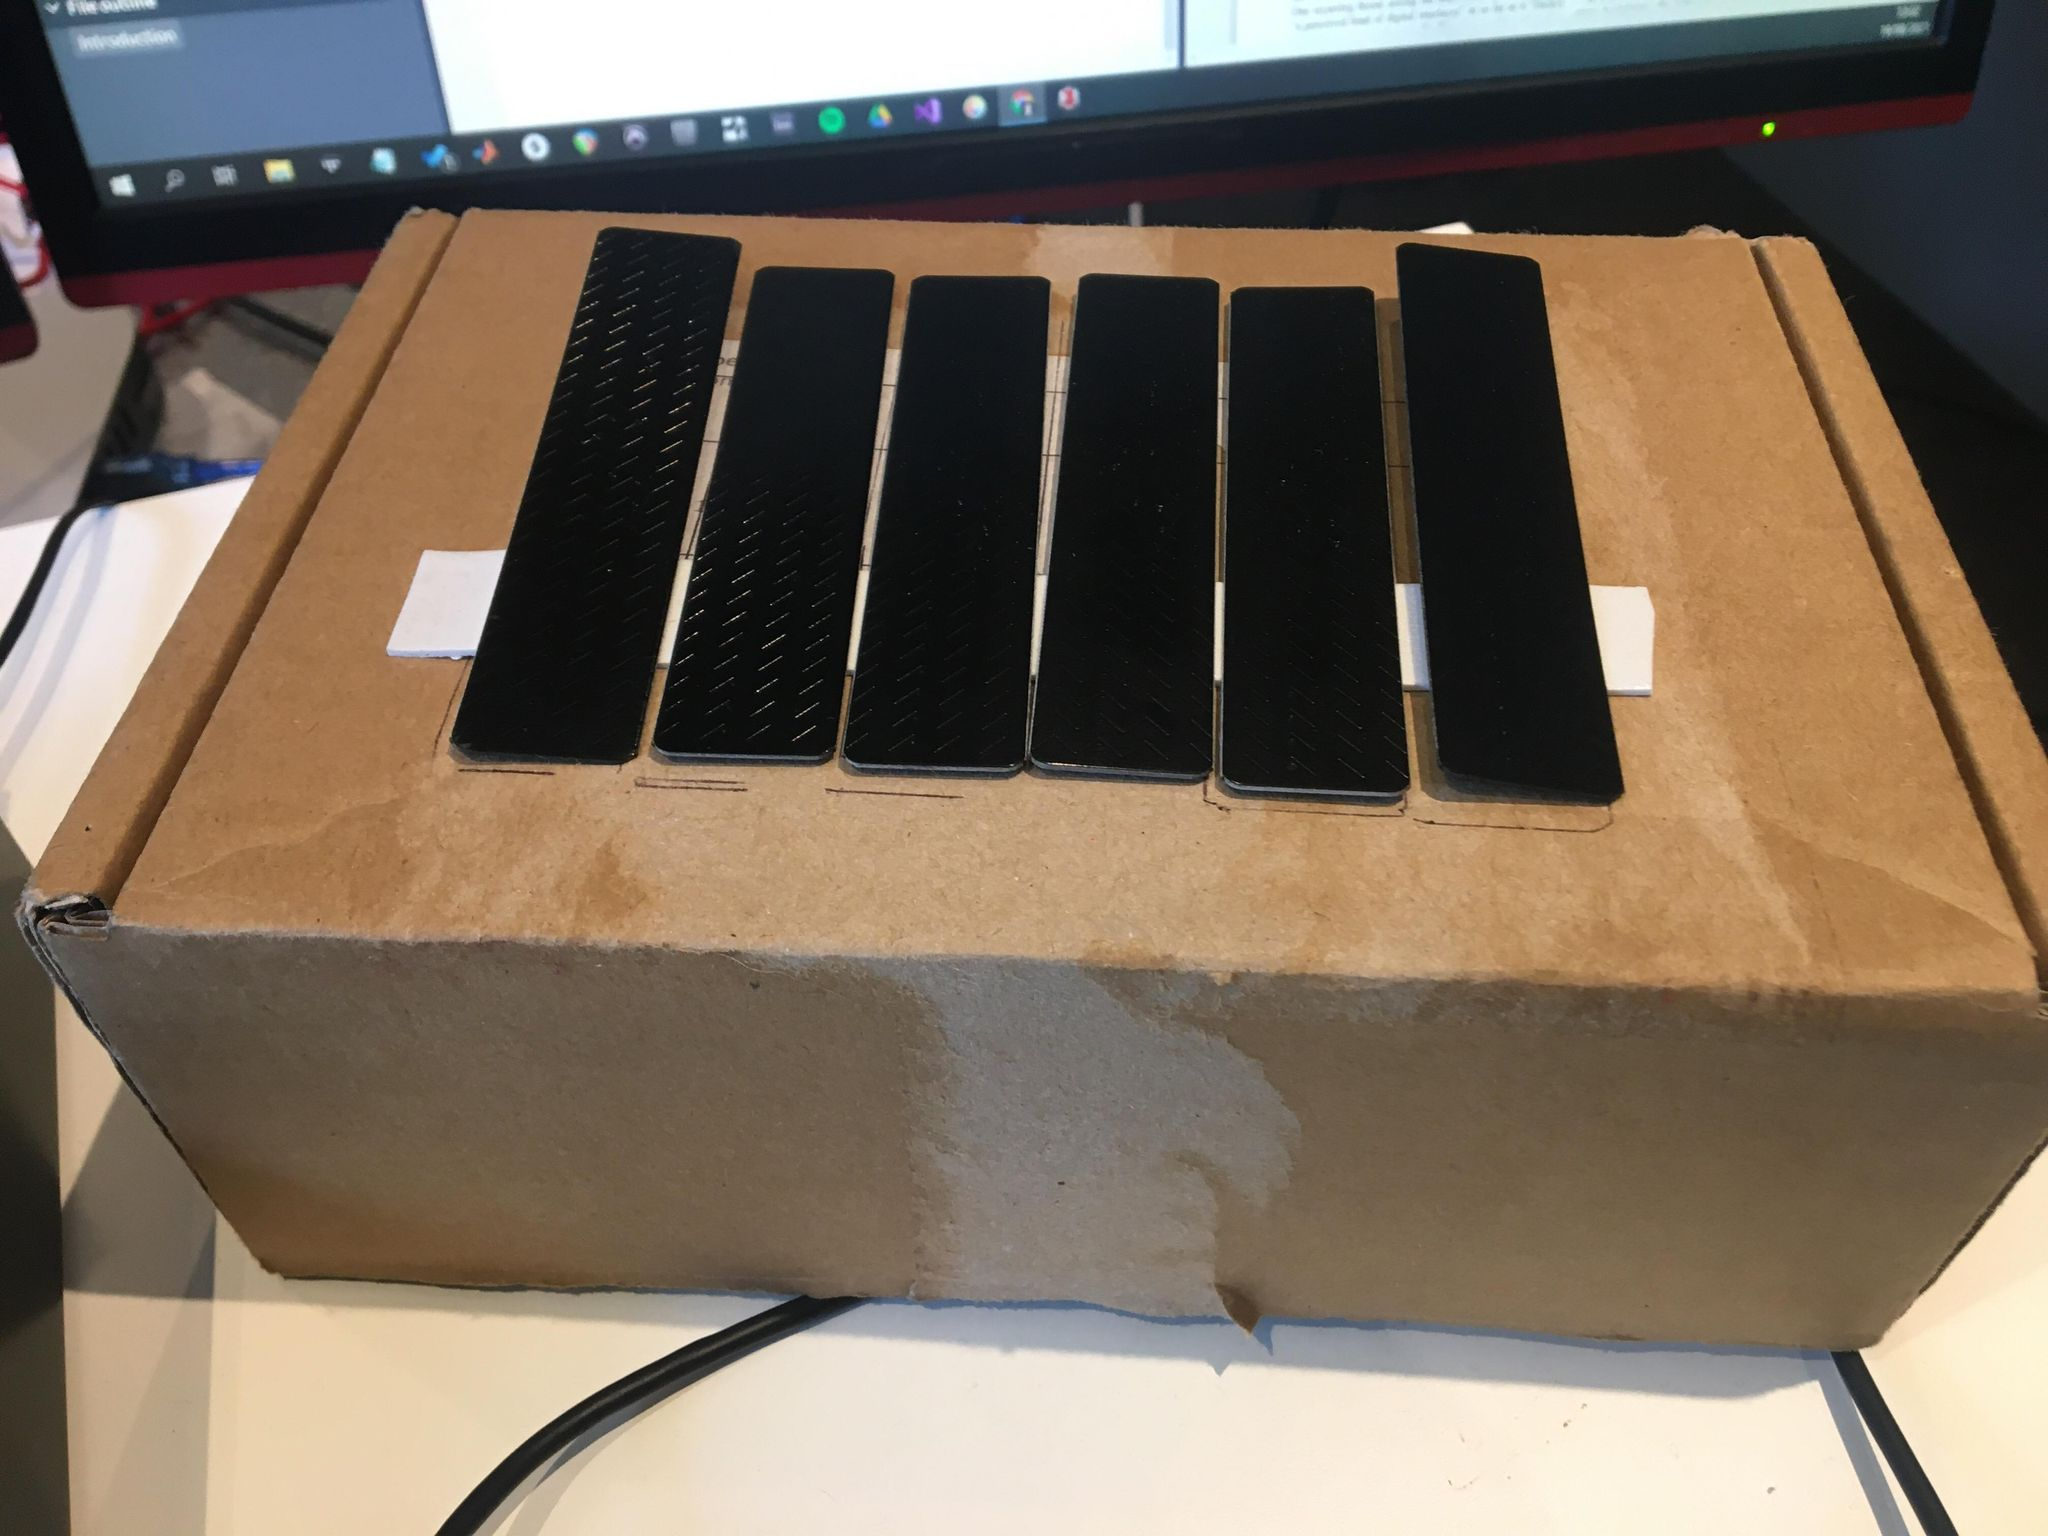
\includegraphics[scale=0.12]{Images/prototype.jpg}
    \caption{Basic proto-prototype.}
    \label{fig:protoprototype}
\end{figure}

This proto-prototype consisted of a small cardboard box that contained the main Bela, and a Trill Hub, with the Trill Bar sensors protruding from the top, which was sufficient to confirm that all the functionality was correct. 

\subsection{Choosing a guitar}
The width of string regions on a typical 6 string guitar is roughly 0.73cm. This may cause the width of each string zone to be quite small, and, at least, reduce the area for possible for pitch bends. This may also have presented a possible frustrating experience for the user, where it may have be to deliver precise finger movements.

Intention not mapping properly to outcome is likely to be frustrating for users. 

This is why, a seven string guitar was used as the basis for the prototype. Although, the prototype does fundamentally have a six string topology, the additional width per string allows for greater margin of error in finger placement. Although no direct comparison to a six-string has been made, this appears to help in the playablility of the prototype.

\subsection{Fitting the sensors}

To fit the sensors to the guitar required a few steps of minor carpentry. Because the Trill sensors have a substantial Grove connector on the rear as can be seen in Figure \ref{fig:trill_picture}. This meant that there had to be a hole cut on each of the frets that were to have sensors mounted. This was achieved by the use of a drill. 

Furthermore, the fret boards of typical guitars are not flat, and thus required sanding to accommodate the flat figure of the Trill sensors.

Additionally, the Trill sensors have their small chip protruding from the rear, which make mounting the sensors flush to the fret board difficult, so a corresponding area on each of the frets was extracted with a drill, such that each sensor was able to lie flush with the fret board. 

\section{Evaluation}

\subsection{Practice-as-research}

This prototype has been evaluated with the use of a \textit{practice-as-research} methodology. This evaluative methodology has been chosen for a number of reasons, first of all being the lingering presence of the COVID-19 pandemic which makes in-person user testing very difficult. Furthermore, it offers a unique lens though which to evaluate this prototype. 

Practice-as-research is an extension of the \textit{research through design} methodology presented in \cite{gaver_what_2012}, which is described as the ``the inference of generalisable principles from a set of design artifacts" \citep{martelloni_guitar_2021}.

In \cite{martelloni_guitar_2021}'s work, the authors highlight the following benefits of practice-as-research, which are logical extensions of the benefits of \cite{gaver_what_2012}'s work. 

These benefits include the affordance of \textit{pre-paradigmatic research}, which is beneficial because the artefact can be evaluated outside of an established set of rules and standards, and this diversity of analysis, Gaver argues, is beneficial to the scientific and research effort.     

Secondly, \cite{martelloni_guitar_2021} highlight a second benefit, put forth by \cite{carey_reection_2016}. This is shown by the concept of the \textit{bricolage} approach to research. This means that ``there is quick feedback on the design, as evaluation and prototyping are brought forward in parallel by the same person or the same group of people". This may mean tighter, and more effective circles of design iteration.

To perform this practice-as-research, the author has used the prototype to compose a new song. This presents an ecologically valid situation for the prototype (in a music studio, in the hands of a guitarist), as well as the benefits listed above.

The piece is available to listen to \href{https://drive.google.com/file/d/1AR7ZPBJgG3uJql0nhqeoFNKMg3zadOTz/view?usp=sharing}{\textbf{here}}. 

The piece was composed using Ableton Live 11 for Microsoft Windows 10. This was chosen since the software has native MPE support \citep{ableton_mpe_2021}. It would still be possible to complete the composition in another DAW which does not have native MPE support, but this would require creating 16 instances of each software instrument, each with a unique MIDI channel, to take advantage of the prototype's MPE functionality. It would also make editing software instrument parameters extremely cumbersome since each of the 16 instances would need to be manually updated individually. Using a DAW with native MPE support avoid this. 

In the following sections we will be exploring a critical analysis of the process in the creation of the author's composition, with respect to the role that the prototype played, and how it changed the way the track was composed. 

\subsubsection{Sound design}
In the composition of the piece, the first thing that was a barrier to creativity was the size of the palette of sounds available that takes advantage of the MPE features of the prototype. The author had developed a preset for Ableton's \textit{Wavetable} synthesizer for debugging and development of the prototype, but beyond this, there did not exist a large palette of sounds to draw from. 

To solve this, composition was stopped, and the author performed a sound design session, creating a set of 16 sounds which take advantage of both the aftertouch and pitch bend abilities of the controller. This step made the process of composition much more straightforward, and less frustrating. 

Sounds that employ the full feature-set of this prototype are typically legato, that map aftertouch to amplitude and brightness (usually by mapping to a low-pass filter cutoff frequency). One typically expects the pitch bend range to be roughly -2 to +2 semitones, which is typical, however there are more experimental sounds that fully employ the pitch bend feature of the prototype, mapping from -24 to +24 semitones. 

\subsubsection{Playing the parts}
The actual prototype is overall quite expressive, and perceivably offers a high degree of fine control over aftertouch and pitch bend features. However, since it was a novel instrument to the author, much of the `muscle memory' that had built up as a traditional guitarist was not as directly translatable as was expected. This meant that performing some parts of the composition such as the lead line, had to be performed a number of times to record a performance that was free of mistakes. 

\subsubsection{Composition}
Overall, the process of composition was subjectively very removed from using a typical non-MPE MIDI controller.

% Why it was easier?
% Why was it more difficult?
% Why it was more inspiring?
In the following ways, the prototype was more creatively inspiring than a non-MPE controller.
 
With the appropriate MPE enabled software instruments, the individual note expression made for a novel experience in comparison to the author's previous experience inputting MIDI into a DAW. This novelty perceivably was in itself a component of the success of the instrument, but this does not speak to it's specific nature that much. 

Speaking directly as a function of the individual note expression, this was able to create much more idiosyncratic synthesizer recordings, that would be incredibly tedious to manually program with a mouse. The lead line of the given composition is a prime example of this. Within the four bar loop of the main theme, each note event is completely unique with respect to its duration and aftertouch envelope. This has the subjective effect of creating a more `organic' or `human' feeling in the music, which represents a successful implementation of the MPE techniques.

% Why it was less inspiring?
However, the composition process was made more cumbersome with the use of the prototype, insofar as the author's muscle memory had not completely entrained with the nature of the instrument yet, and this nature of being unable to convert intention to reality was at times frustrating. This can be understood as a natural function of it being a new instrument, but one of the aims of this prototype is to be able to more directly translate previously available muscle memory to the MIDI domain. This offers a direction for improvement in future iterations of the design.

Though the novelty was very inspiring, this layer of frustration prohibited some level of creativity.

% Why it was less practical? 
In comparison to the desktop, keyboard style MIDI controllers, guitar-like MIDI controllers, MPE enabled or otherwise, may be less suitable for studio applications than previously thought. 

In a practical sense, having a keyboard on the desk in front of the musician or producer is a `natural', and well established studio practice. However, the practicalities of balancing a guitar on one's lap, while leaning over to try and start recording, or editing MIDI, after a few hours in the studio is more creatively draining than simply accessing a MIDI controller that is at rest on the desktop. 

Though this is perhaps a minor observation, if our goal is to optimise the creative potential for users, this is a problem worth examining. 

% Talk about how it's harder to express your ideas, because it requires you to be able to play the instrument well, and you're not perfect at playing the instrument well yet, which made it more frustrating than necessary. 

% What are some of it's overall successes? 
Subjectively, the author believes that the addition of authentic human expression in the composition is successful. This links to studies such as \cite{witek_syncopation_2014}, which discuss the effect of groove and imperfect timing on the increased enjoyment of music, at least in particular styles. 

It was also interesting that, since editing many notes of MPE material in post-production is laborious and cumbersome, this invited performing more takes of the performance to get a satisfactory recording. This practice supports musicianship in favour of over-editing, which can often make for a more authentic musical experience. 

% !!!!!!!!!!!!!!!!!! Can we do a COGNITIVE WALK THROUGH???????? !!!!!

% WHAT KIND OF ERROR IS THE STRING MISMATCH ERROR????? NORMAN!

% HOW DO WE STACK UP AGAINST OUR GOAL OF MARTELLONI'S DIGITAL PHONBIA ETC???

% How does it contrast to using a typical MIDI keyboard?


% % What would you do to fix the issues you raised above?
% KEY ISSUES:
% - difficult to hold in sat down in the studio
% - not matchign muscle memoery from tradiditonal guitar
% - not currently having open string triggers, which does not support traditional guitar-style strumming or playing. 
% - creatively draining in the long term (of a session).
% - needs wires tidying up. 
% - wants haptic feedback on the neck, insofar as you can 'feel' the strings like you can on a normal guitar. This would probably help with the transition, but this may conflict with the expression of the strings. Maybe just put haptic feedback on the string boundaries. 

% KEY BENEFITS:
% - musically expressive and more authentic performances. 
% - fun!
% - supports creativity in the short term
% - pitch bend/vibrato is successful! 

% \subsubsection{Listening and reflection}

% % Okay, so what sort of things do we need to do? Dunno! Um. 

% % Listening. 

% % On listening, it's pretty, uh more human, but you can hear more of the mistakes. 

% % Though I'm not an expert in playing it, it's pretty cool. You need more time to get the shit right. 

% % You need to spend more time practicing with it, which is annoying, but could reap big rewards.

% \subsubsection{Aspects to develop in the next design iteration}


\subsection{Heuristic Evaluation}

To further extend the evaluation of the prototype, we can conduct a heuristic evaluation. Heuristic evaluation is a method for identifying the usability problems in a user interface design \citep{nielsen_usability_1994, nielsen_heuristic_1990}. Since our prototype is indeed a type of user interface, this evaluative process can add some value to this study. 

Heuristic evaluation consists of generally a number of `expert' user interface designers who will assess the system (our prototype) to a number of `heuristics', these are outlined briefly in Appendix \ref{appendix:heuristics}.

By walking step by step through these heuristics we highlight a number of successes of the design, but also elements which could be improved. By highlighting these areas for improvement, we hope to contribute to the better understanding of prototyping this type of NIME for future researchers and practitioners. 

It is noted that not all of the points analysed here relate directly to the MPE functionality of the prototype, but the frustrations of points raised will cumulatively impact the prototype's ability to support creativity in general, and creating a device that is supportive of creativity is one of the goals of this study.

% MENTION THAT YOU'RE AWARE THAT MAYBE THIS IS A WONKY WAY TO EVALUATE NIME. MAYBE YOU SHOULD ALSO EVALUATE WITH RESPECT TO SOME MORE NIMEY LITERATURE?

Furthermore, the author notes the work of \cite{rodger_what_2020}, noting that traditional HCI evaluation of NIME is not necessarily the most effective. \cite{rodger_what_2020} argue that since instruments are more completely described with reference to their context. The affordances of any one instrument interact with and constrain other affordances and processes of its interconnected systems, for example connected DAWs and digital synthesizers. The authors summarise the issue neatly with the following quotation:

\begin{quote}
    ``Instruments can do and mean many different things that are not easily delimited by a predetermined functional teleology, and this is affected by their evolution among other instruments and musical practices." \\ 
    \hspace*{\fill} \textit{\cite{rodger_what_2020}}
\end{quote}

Traditional HCI evaluation makes the implicit assumption that precision, control and accuracy are valued \cite{rodger_what_2020}, but many subjectively successful NIME do not conform to this assumption \cite{gurevich_expression_2007}. However, this instrument \textit{does} happen to value control and precision, and since it is a new type of instrument, the following heuristic evaluation offers a broad-strokes analysis of the benefits and shortcomings of the design as it stands. 

\subsubsection{Visibility of system status}
Since the system only has a limited set of states, either `on' or `off', it is tempting to imagine that there is not need for system feedback beyond a simple power LED. However, this is only a prototype, and as the feature-set grows to incorporate strumming modes, and other input modes, users should be able to know that the system is in fact in the right `mode'. This will help avoid mode errors, which can be very frustrating for a user. One might imagine a user on stage with this digital instrument, about to perform a solo, but their instrument not properly signify which mode it was in, and result in an undesired output, and unhappy concert-goers. 

Currently, while the prototype is indeed a prototype and bound to wired studio use, the power indicator on the Bela board is likely sufficient, but as the features grow, this will change and more sophisticated signifiers of mode will be required.



\subsubsection{Match between system and the real world}
Since this is a new system, which does not behave the same way as a `traditional' guitar, we say there is an unnatural mapping between our prototype and the traditional guitar. In this sense there is arguably not a great match between the system and the `real world' of the traditional guitar, which some users may find jarring.

We might consider two solutions to this. Either, the prototype should support traditional guitar style playing, so that users can use the system in a way which matches up with their expectations, or it is somehow able to make it clear to the users what \textit{is} possible with the prototype and what is \textit{not}. This could be done with forcing functions by having definitively no place to strum, and thus prohibit this behaviour, for example. 

However the latter is not conducive to this study's goal of creating a system which is conducive to creativity. A system that aims to foster creativity should have affordances for self-expression that support users in as many ways as possible. 

\subsubsection{User control and freedom}
This heuristic is effectively a question of whether the device supports undoing mistakes, or cancelling unwanted tasks. 

This heuristic is not so applicable to our prototype in it's current state just like heuristic \textit{1)}. However this is something to be aware of in future iterations. If a user accidentally changes mode, it should take one \textit{easily identifiable} `click' or button press to get back to where they were. 

\subsubsection{Consistency and standards}
This prototype implements MIDI, which is a standardized digital protocol. This prototype should, and broadly does, apply this standard. However, this is necessary but not sufficient. Most MIDI instruments exhibit a `plug-and-play' functionality, which means that as soon as they are plugged into the computer, they immediately begin to work. This is a convention that the prototype does follow by using the Bela `Run project on boot' functionality as can be seen in Figure \ref{fig:runonboot}. 

\begin{figure}[h]
    \centering
    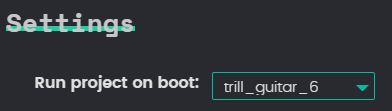
\includegraphics[scale=0.8]{Images/run on boot.png}
    \caption{The Bela IDE's `Run project on boot' functionality.}
    \label{fig:runonboot}
\end{figure}

However, the Bela ambiguously identifies its MIDI port as `Midi function', as can be see in Figure \ref{fig:midifunction}. It is a typical practice for MIDI devices to identify themselves with a helpful name such as "AugGuitar Prototype V1.0" for example.

\begin{figure}[h]
    \centering
    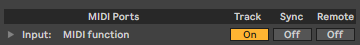
\includegraphics[scale=0.8]{Images/midi function.png}
    \caption{The Bela MIDI device appearing with as `MIDI Function' in the MIDI ports list of Ableton Live 10. }
    \label{fig:midifunction}
\end{figure}

This is a type of \textit{external} inconsistency \citep{nielsen_heuristic_1990}, and is likely to confuse users on the first time using it, which may impede their creativity. 

\subsubsection{Error prevention}

As highlighted in the section above, the lack of visual and haptic (for example emulating the physical sensation of strings across the sensors) feedback as to the position of string centres does not support error prevention particularly well. 

It is not very forgiving of accidental incorrect finger placement, and only permits users who already have a muscle memory of the position of the strings to work without error. Despite being the developer of the prototype, even the author does not possess this ability. 

The addition of haptic feedback (e.g. dummy strings across the sensors) would also be more supportive of visually impaired users, which would be beneficial. 

On the other hand, the prototype's pitch bend functionality is more successful in this sense. Where the prototype does not bend the note, regardless of initial touch location and the addition of the $\alpha$ exponent in expression \ref{eq:pitchbend} helps in the reduction of unwanted pitch bends. This should help make the experience less frustrating, and ultimately more creatively supportive. 

\subsubsection{Recognition rather than recall}
There are few things to have to remember about the current design with respect to it's usability. Insofar as there are no deep menus to traverse. Thus, this heuristic is less applicable to the prototype than some of the others. 

\subsubsection{Flexibility and efficiency of use}
Under heuristic \textit{2)} we touched on a point about some users that will want, or expect, the prototype to function like a traditional guitar. In this way, the prototype is not flexible, since it only supports one style of playing. To amend this, a greater number of playing styles could be supported, which would increase the flexibility and usability of the prototype. 

\subsubsection{Aesthetic and minimal design}
Currently the prototype is very minimal indeed, and certainly does not show superfluous information to the user. It might be argued that the vestigial volume and tone knobs, and pick up selector tack against this heuristic, but they naturally would not continue into later iterations of the design since they serve no functional purpose in the system.

\subsubsection{Help users recognize, diagnose and recover from errors}
Currently, the prototype offers implicit feedback to slips where the wrong note is pushed, because the wrong note will sound. However this point is somewhat of a triviality.

As the prototype develops, it should offer more sophisticated feedback to general troubleshooting issues such as drivers failing to load, etc. However, issues like this are not the concern of this prototype. 

% IT ALSO COULD BE INTERESTING TO SHOW AN APP THAT SHOWS THE TOUCH LOCATIONS IN REAL TIME JUST LIKE IN THE BELA DEMOS. 

\subsubsection{Help and documentation}
This heuristic is also less applicable to this prototype. The interface being a guitar shape is reasonably self-evident, but as the feature-set grows supporting documentation about driver installation should be created as required. 
 % GAHHH NOT REALLY APPLICAABLE! ANYWAY TIME FOR A BREAKKKKKKKKKKK. 



% However as the system is reasonably complex, and has a number of sensors which may be incorrectly connected or otherwise faulty, we might imagine a use being confused at the lack of feedback if something 









\section{Summary and Conclusion}

To conclude, we have explored how capacitive touch sensors can be applied to the guitar to create an expressive MPE instrument. The interaction design for this instrument is not yet perfected, but offers a direction for further development.

We have proposed a framework for mathematically interpreting the sensor data which can scale to any number of frets or strings, which means that this system can scale indefinitely to accommodate any sized system.

We have evaluated how the prototype is overall effective in delivering the desired expressive features, but requires some refinement to be truly creatively liberating. 





\section*{Acknowledgement}
I would like to thank everyone in the \textbf{\href{http://www.eecs.qmul.ac.uk/}{C4DM}} at QMUL, each of which in their own way has helped to inform my understanding and interest in digital audio, music and human-centred design. In particular Mathieu Barthet, Andrew McPherson, Paul Curzon and Sophie Skatch who have all been instrumental in supporting my learning in the modules they teach. 

In particular, Mathieu Barthet has been an extremely attentive and supportive supervisor to this project and I thank him immensely for his support on this journey. 

% \bibliographystyle{IEEEtran}
% \bibliography{IEEEabrv,references}
% \Urlmuskip=0mu plus 1mu\relax
\bibliographystyle{agsm}
\bibliography{references}

\clearpage

\begin{appendices}

\section{Final Prototype Photos}
\label{appendices:guitarimages}
\centering
\begin{figure}[h]
    \centering
    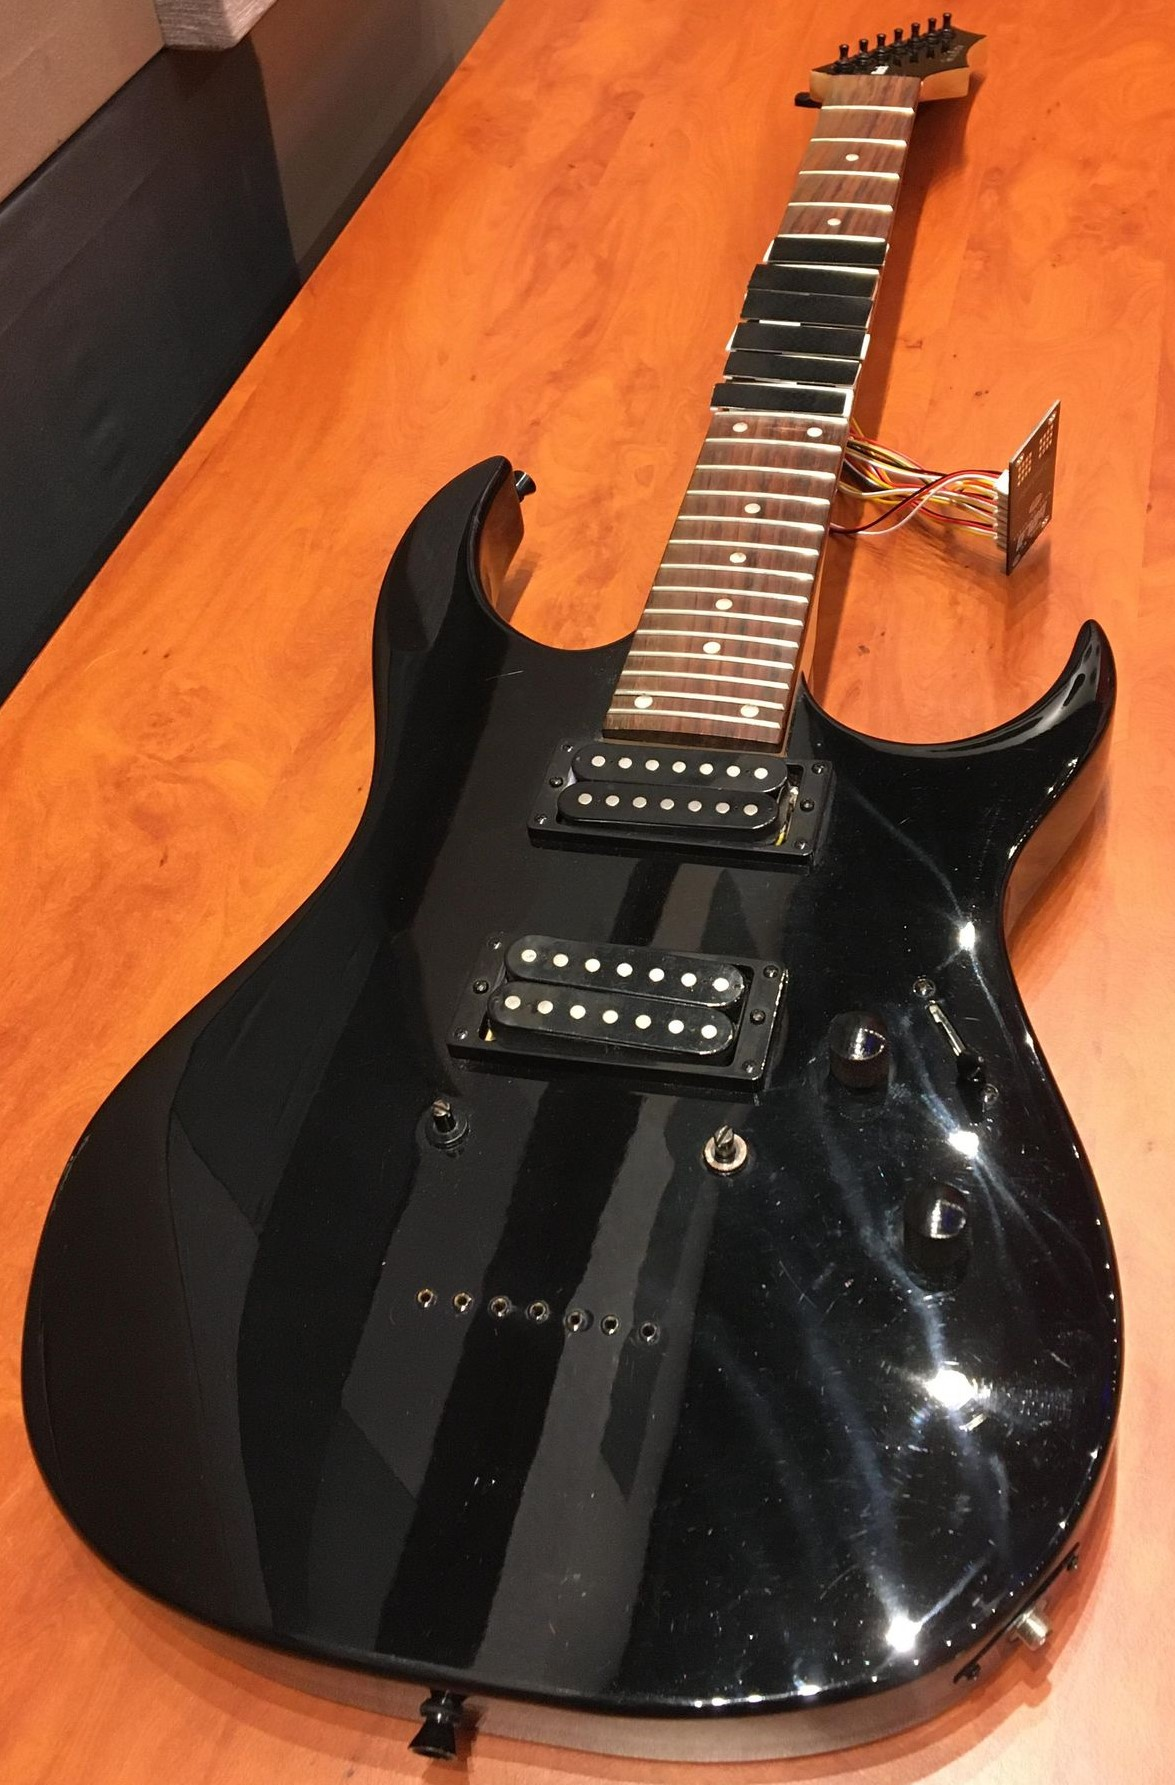
\includegraphics[scale=0.25]{Images/guitargui.jpg}
    \caption{Front of the prototype.}
    \label{fig:my_label}
\end{figure}
\begin{figure}[h]
    \centering
    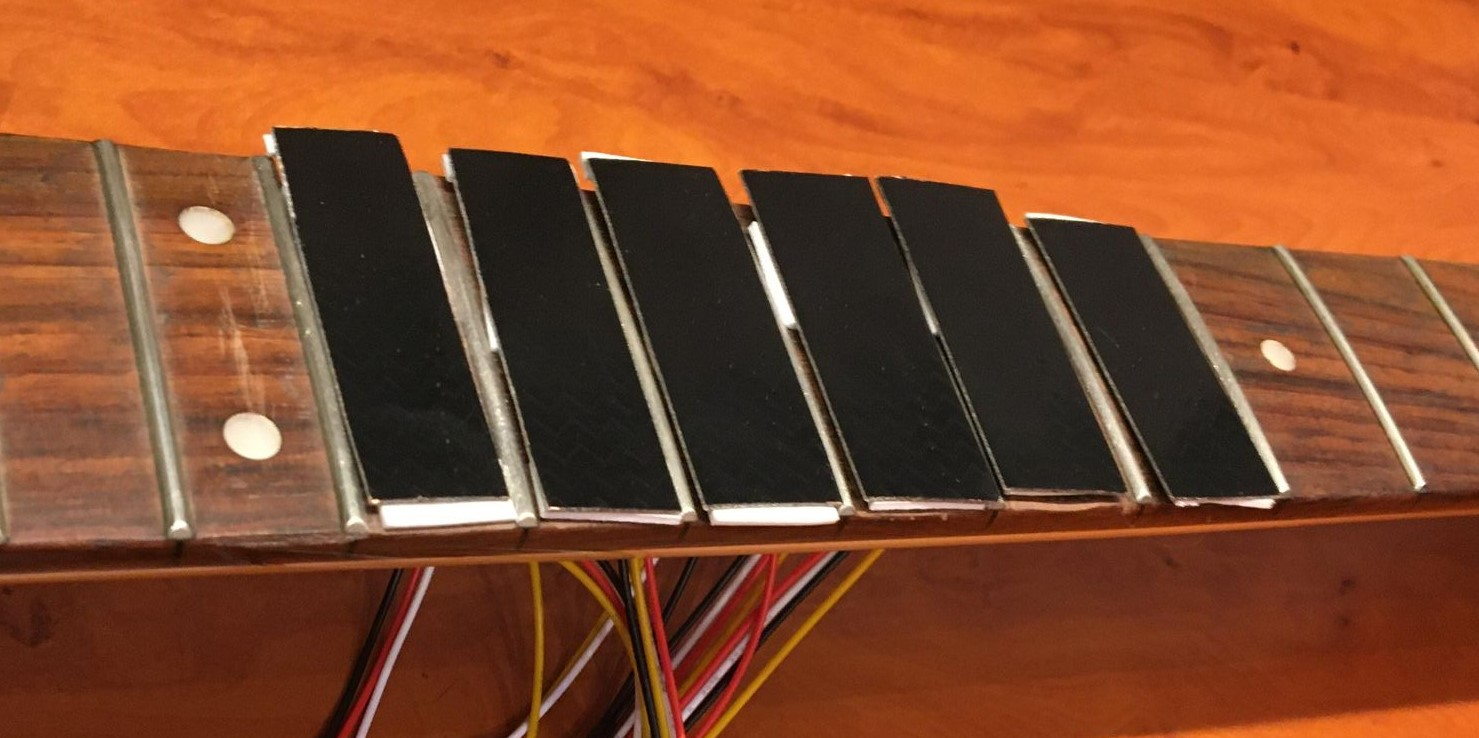
\includegraphics[scale=0.2]{Images/neck.jpg}
    \caption{Close-up of neck sensors.}
    \label{fig:my_label}
\end{figure}
\begin{figure}[h]
    \centering
    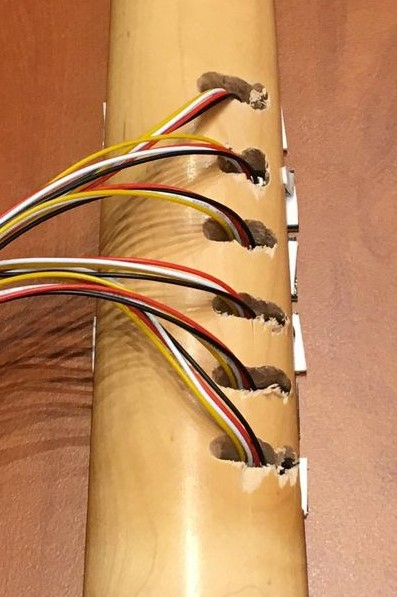
\includegraphics[scale=0.6]{Images/back.jpg}
    \caption{Back of the neck, to show I2C wiring to the sensors.}
    \label{fig:my_label}
\end{figure}

\clearpage
\section{Nielsen Usability Heuristics}
\label{appendix:heuristics}
\begin{enumerate}
    \item \textbf{Visibility of system status}: does the design keep the user informed about what is going on? 
    \item \textbf{Match between the system and the real world}: does the design follow real-world conventions and use phrases and concepts which are familiar to the user?
    \item \textbf{User control and freedom}: are users able to easily correct mistakes? This helps foster a sense of freedom and confidence in the user. 
    \item \textbf{Consistency and standards}: does the design follow platform and industry standards/conventions?
    \item \textbf{Error prevention}: it is important to let the user know when things have gone wrong, but it is even better to help prevent errors in the first place. Does the design help prevent common errors from happening?
    \item \textbf{Recognition rather than recall}: does the design minimise the user's memory load by making the interface as available as possible? Does the user have to remember different parts of the interface are hidden in deep context menus?
    \item \textbf{Flexibility and efficiency of use}: does the design offer shortcuts to expert users such that they may be able to speed up their workflow, but at the same time allowing novice users to access all the features at their own pace?
    \item \textbf{Aesthetic and minimal design}: does the interface contain information which is not needed? Interfaces should aim to minimise irrelevant information, since this reduces the relative visibility of important, relevant information.
    \item \textbf{Help users recognise, diagnose and recover from errors}: are errors expressed in plain and simple language? Does the system precisely indicate problems and suggest solutions?
    \item \textbf{Help and documentation}: does the system require additional documentation? Though it's best if the system doesn't need additional explanation, if this \textit{is} required, does the system offer this help?
\end{enumerate}









\end{appendices}


\end{document}

